% Options for packages loaded elsewhere
% Options for packages loaded elsewhere
\PassOptionsToPackage{unicode}{hyperref}
\PassOptionsToPackage{hyphens}{url}
\PassOptionsToPackage{dvipsnames,svgnames,x11names}{xcolor}
%
\documentclass[
  italian,
  a4paper,
]{article}
\usepackage{xcolor}
\usepackage{amsmath,amssymb}
\setcounter{secnumdepth}{5}
\usepackage{iftex}
\ifPDFTeX
  \usepackage[T1]{fontenc}
  \usepackage[utf8]{inputenc}
  \usepackage{textcomp} % provide euro and other symbols
\else % if luatex or xetex
  \usepackage{unicode-math} % this also loads fontspec
  \defaultfontfeatures{Scale=MatchLowercase}
  \defaultfontfeatures[\rmfamily]{Ligatures=TeX,Scale=1}
\fi
\usepackage{lmodern}
\ifPDFTeX\else
  % xetex/luatex font selection
\fi
% Use upquote if available, for straight quotes in verbatim environments
\IfFileExists{upquote.sty}{\usepackage{upquote}}{}
\IfFileExists{microtype.sty}{% use microtype if available
  \usepackage[]{microtype}
  \UseMicrotypeSet[protrusion]{basicmath} % disable protrusion for tt fonts
}{}
\makeatletter
\@ifundefined{KOMAClassName}{% if non-KOMA class
  \IfFileExists{parskip.sty}{%
    \usepackage{parskip}
  }{% else
    \setlength{\parindent}{0pt}
    \setlength{\parskip}{6pt plus 2pt minus 1pt}}
}{% if KOMA class
  \KOMAoptions{parskip=half}}
\makeatother
% Make \paragraph and \subparagraph free-standing
\makeatletter
\ifx\paragraph\undefined\else
  \let\oldparagraph\paragraph
  \renewcommand{\paragraph}{
    \@ifstar
      \xxxParagraphStar
      \xxxParagraphNoStar
  }
  \newcommand{\xxxParagraphStar}[1]{\oldparagraph*{#1}\mbox{}}
  \newcommand{\xxxParagraphNoStar}[1]{\oldparagraph{#1}\mbox{}}
\fi
\ifx\subparagraph\undefined\else
  \let\oldsubparagraph\subparagraph
  \renewcommand{\subparagraph}{
    \@ifstar
      \xxxSubParagraphStar
      \xxxSubParagraphNoStar
  }
  \newcommand{\xxxSubParagraphStar}[1]{\oldsubparagraph*{#1}\mbox{}}
  \newcommand{\xxxSubParagraphNoStar}[1]{\oldsubparagraph{#1}\mbox{}}
\fi
\makeatother

\usepackage{color}
\usepackage{fancyvrb}
\newcommand{\VerbBar}{|}
\newcommand{\VERB}{\Verb[commandchars=\\\{\}]}
\DefineVerbatimEnvironment{Highlighting}{Verbatim}{commandchars=\\\{\}}
% Add ',fontsize=\small' for more characters per line
\usepackage{framed}
\definecolor{shadecolor}{RGB}{241,243,245}
\newenvironment{Shaded}{\begin{snugshade}}{\end{snugshade}}
\newcommand{\AlertTok}[1]{\textcolor[rgb]{0.68,0.00,0.00}{#1}}
\newcommand{\AnnotationTok}[1]{\textcolor[rgb]{0.37,0.37,0.37}{#1}}
\newcommand{\AttributeTok}[1]{\textcolor[rgb]{0.40,0.45,0.13}{#1}}
\newcommand{\BaseNTok}[1]{\textcolor[rgb]{0.68,0.00,0.00}{#1}}
\newcommand{\BuiltInTok}[1]{\textcolor[rgb]{0.00,0.23,0.31}{#1}}
\newcommand{\CharTok}[1]{\textcolor[rgb]{0.13,0.47,0.30}{#1}}
\newcommand{\CommentTok}[1]{\textcolor[rgb]{0.37,0.37,0.37}{#1}}
\newcommand{\CommentVarTok}[1]{\textcolor[rgb]{0.37,0.37,0.37}{\textit{#1}}}
\newcommand{\ConstantTok}[1]{\textcolor[rgb]{0.56,0.35,0.01}{#1}}
\newcommand{\ControlFlowTok}[1]{\textcolor[rgb]{0.00,0.23,0.31}{\textbf{#1}}}
\newcommand{\DataTypeTok}[1]{\textcolor[rgb]{0.68,0.00,0.00}{#1}}
\newcommand{\DecValTok}[1]{\textcolor[rgb]{0.68,0.00,0.00}{#1}}
\newcommand{\DocumentationTok}[1]{\textcolor[rgb]{0.37,0.37,0.37}{\textit{#1}}}
\newcommand{\ErrorTok}[1]{\textcolor[rgb]{0.68,0.00,0.00}{#1}}
\newcommand{\ExtensionTok}[1]{\textcolor[rgb]{0.00,0.23,0.31}{#1}}
\newcommand{\FloatTok}[1]{\textcolor[rgb]{0.68,0.00,0.00}{#1}}
\newcommand{\FunctionTok}[1]{\textcolor[rgb]{0.28,0.35,0.67}{#1}}
\newcommand{\ImportTok}[1]{\textcolor[rgb]{0.00,0.46,0.62}{#1}}
\newcommand{\InformationTok}[1]{\textcolor[rgb]{0.37,0.37,0.37}{#1}}
\newcommand{\KeywordTok}[1]{\textcolor[rgb]{0.00,0.23,0.31}{\textbf{#1}}}
\newcommand{\NormalTok}[1]{\textcolor[rgb]{0.00,0.23,0.31}{#1}}
\newcommand{\OperatorTok}[1]{\textcolor[rgb]{0.37,0.37,0.37}{#1}}
\newcommand{\OtherTok}[1]{\textcolor[rgb]{0.00,0.23,0.31}{#1}}
\newcommand{\PreprocessorTok}[1]{\textcolor[rgb]{0.68,0.00,0.00}{#1}}
\newcommand{\RegionMarkerTok}[1]{\textcolor[rgb]{0.00,0.23,0.31}{#1}}
\newcommand{\SpecialCharTok}[1]{\textcolor[rgb]{0.37,0.37,0.37}{#1}}
\newcommand{\SpecialStringTok}[1]{\textcolor[rgb]{0.13,0.47,0.30}{#1}}
\newcommand{\StringTok}[1]{\textcolor[rgb]{0.13,0.47,0.30}{#1}}
\newcommand{\VariableTok}[1]{\textcolor[rgb]{0.07,0.07,0.07}{#1}}
\newcommand{\VerbatimStringTok}[1]{\textcolor[rgb]{0.13,0.47,0.30}{#1}}
\newcommand{\WarningTok}[1]{\textcolor[rgb]{0.37,0.37,0.37}{\textit{#1}}}

\usepackage{longtable,booktabs,array}
\newcounter{none} % for unnumbered tables
\usepackage{calc} % for calculating minipage widths
% Correct order of tables after \paragraph or \subparagraph
\usepackage{etoolbox}
\makeatletter
\patchcmd\longtable{\par}{\if@noskipsec\mbox{}\fi\par}{}{}
\makeatother
% Allow footnotes in longtable head/foot
\IfFileExists{footnotehyper.sty}{\usepackage{footnotehyper}}{\usepackage{footnote}}
\makesavenoteenv{longtable}
\usepackage{graphicx}
\makeatletter
\newsavebox\pandoc@box
\newcommand*\pandocbounded[1]{% scales image to fit in text height/width
  \sbox\pandoc@box{#1}%
  \Gscale@div\@tempa{\textheight}{\dimexpr\ht\pandoc@box+\dp\pandoc@box\relax}%
  \Gscale@div\@tempb{\linewidth}{\wd\pandoc@box}%
  \ifdim\@tempb\p@<\@tempa\p@\let\@tempa\@tempb\fi% select the smaller of both
  \ifdim\@tempa\p@<\p@\scalebox{\@tempa}{\usebox\pandoc@box}%
  \else\usebox{\pandoc@box}%
  \fi%
}
% Set default figure placement to htbp
\def\fps@figure{htbp}
\makeatother


% definitions for citeproc citations
\NewDocumentCommand\citeproctext{}{}
\NewDocumentCommand\citeproc{mm}{%
  \begingroup\def\citeproctext{#2}\cite{#1}\endgroup}
\makeatletter
 % allow citations to break across lines
 \let\@cite@ofmt\@firstofone
 % avoid brackets around text for \cite:
 \def\@biblabel#1{}
 \def\@cite#1#2{{#1\if@tempswa , #2\fi}}
\makeatother
\newlength{\cslhangindent}
\setlength{\cslhangindent}{1.5em}
\newlength{\csllabelwidth}
\setlength{\csllabelwidth}{3em}
\newenvironment{CSLReferences}[2] % #1 hanging-indent, #2 entry-spacing
 {\begin{list}{}{%
  \setlength{\itemindent}{0pt}
  \setlength{\leftmargin}{0pt}
  \setlength{\parsep}{0pt}
  % turn on hanging indent if param 1 is 1
  \ifodd #1
   \setlength{\leftmargin}{\cslhangindent}
   \setlength{\itemindent}{-1\cslhangindent}
  \fi
  % set entry spacing
  \setlength{\itemsep}{#2\baselineskip}}}
 {\end{list}}
\usepackage{calc}
\newcommand{\CSLBlock}[1]{\hfill\break\parbox[t]{\linewidth}{\strut\ignorespaces#1\strut}}
\newcommand{\CSLLeftMargin}[1]{\parbox[t]{\csllabelwidth}{\strut#1\strut}}
\newcommand{\CSLRightInline}[1]{\parbox[t]{\linewidth - \csllabelwidth}{\strut#1\strut}}
\newcommand{\CSLIndent}[1]{\hspace{\cslhangindent}#1}

\ifLuaTeX
\usepackage[bidi=basic,shorthands=off]{babel}
\else
\usepackage[bidi=default,shorthands=off]{babel}
\fi
\ifLuaTeX
  \usepackage{selnolig} % disable illegal ligatures
\fi


\setlength{\emergencystretch}{3em} % prevent overfull lines

\providecommand{\tightlist}{%
  \setlength{\itemsep}{0pt}\setlength{\parskip}{0pt}}



 


\usepackage{graphicx}
\graphicspath{ {../Report/} }
\usepackage{fvextra}
\usepackage{hyperref}
\usepackage{xurl}
\hypersetup{breaklinks=true}
\usepackage{fontawesome5}
\usepackage{newunicodechar}
\newunicodechar{👤}{\faUser}
\newunicodechar{📄}{\faFile}
\newunicodechar{🔗}{\faLink}
\newunicodechar{📊}{\faChartBar}
\newunicodechar{🌍}{\faGlobe}
\newunicodechar{✅}{\faCheckCircle}
\newunicodechar{🔹}{\faCaretRight}
\newunicodechar{👈}{\faHandPointLeft}
\newunicodechar{❌}{\faTimes}
\newunicodechar{▶}{\faPlay}
\newunicodechar{μ}{\ensuremath{\mu}}
\newunicodechar{≈}{\ensuremath{\approx}}
\newunicodechar{⚠}{\faExclamationTriangle}
\newunicodechar{≥}{\ensuremath{\geq}}
\newunicodechar{️}{}
\newunicodechar{├}{\textbar}
\newunicodechar{─}{-}
\newunicodechar{└}{\textbar}
\newunicodechar{│}{\textbar}
\usepackage{float}
%\usepackage{caption}
\makeatletter
  \makeatletter
  \AtBeginDocument{%
    \fvset{breaklines=true, breakanywhere=true}%
    \def\listingname{Codice}%
    \providecommand{\thecodelisting}{\arabic{codelisting}}%
    \renewenvironment{codelisting}{%
      \par\medskip\noindent%
      \refstepcounter{codelisting}%
      \def\caption##1{##1\par\noindent\small\listingname~\thecodelisting\par}%
    }{\par\medskip}%
    \RecustomVerbatimEnvironment{verbatim}{Verbatim}{breaklines=true,breakanywhere=true,breaksymbolleft={},breakindent=0pt,fontsize=\small}%
  }
\makeatother
\makeatletter
\@ifpackageloaded{caption}{}{\usepackage{caption}}
\AtBeginDocument{%
\ifdefined\contentsname
  \renewcommand*\contentsname{Indice}
\else
  \newcommand\contentsname{Indice}
\fi
\ifdefined\listfigurename
  \renewcommand*\listfigurename{Elenco delle Figure}
\else
  \newcommand\listfigurename{Elenco delle Figure}
\fi
\ifdefined\listtablename
  \renewcommand*\listtablename{Elenco delle Tabelle}
\else
  \newcommand\listtablename{Elenco delle Tabelle}
\fi
\ifdefined\figurename
  \renewcommand*\figurename{Figura}
\else
  \newcommand\figurename{Figura}
\fi
\ifdefined\tablename
  \renewcommand*\tablename{Tabella}
\else
  \newcommand\tablename{Tabella}
\fi
}
\@ifpackageloaded{float}{}{\usepackage{float}}
\floatstyle{ruled}
\@ifundefined{c@chapter}{\newfloat{codelisting}{h}{lop}}{\newfloat{codelisting}{h}{lop}[chapter]}
\floatname{codelisting}{Lista}
\newcommand*\listoflistings{\listof{codelisting}{Elenco degli Elenchi}}
\makeatother
\makeatletter
\makeatother
\makeatletter
\@ifpackageloaded{caption}{}{\usepackage{caption}}
\@ifpackageloaded{subcaption}{}{\usepackage{subcaption}}
\makeatother
\makeatletter
\definecolor{QuartoInternalColor1}{rgb}{0.70,0.17,0.19}
\definecolor{QuartoInternalColor4}{rgb}{0.00,0.64,0.31}
\definecolor{QuartoInternalColor6}{rgb}{0.60,0.00,0.00}
\definecolor{QuartoInternalColor8}{rgb}{0.20,0.40,0.40}
\definecolor{QuartoInternalColor9}{rgb}{0.60,0.00,1.00}
\definecolor{QuartoInternalColor3}{rgb}{0.00,0.45,0.15}
\definecolor{QuartoInternalColor7}{rgb}{0.00,0.40,0.00}
\definecolor{QuartoInternalColor2}{rgb}{0,0,0}
\definecolor{QuartoInternalColor5}{rgb}{0.38,0.38,0.38}
\makeatother
\usepackage{bookmark}
\IfFileExists{xurl.sty}{\usepackage{xurl}}{} % add URL line breaks if available
\urlstyle{same}
\hypersetup{
  pdftitle={Epstein Files},
  pdflang={it},
  colorlinks=true,
  linkcolor={blue},
  filecolor={Maroon},
  citecolor={Blue},
  urlcolor={Blue},
  pdfcreator={LaTeX via pandoc}}


\title{Epstein Files}
\author{}
\date{}
\begin{document}
\maketitle

\renewcommand*\contentsname{Indice}
{
\setcounter{tocdepth}{4}
\tableofcontents
}

\section{Epstein Files}\label{epstein-files}

\begin{figure}[H]

{\centering \pandocbounded{
\includegraphics[keepaspectratio]{Images/FirstAmendment.jpg}}

}

\caption{image}

\end{figure}%

\subsection{Introduzione}\label{introduzione}

Gli \href{https://en.wikipedia.org/wiki/Epstein_files}{Epstein Files}
sono i documenti investigativi riguardanti il notorio finanziere
pedofilo Jeffrey Epstein. La totalità di questi file occupa, ad oggi
18-03-2026, all'incirca 300 GB.

\subsubsection{Argomento di Ricerca}\label{argomento-di-ricerca}

Come vedremo meglio introducendo il dataset ¬ Molte entità citate nei
file sono o censurate o citate vagamente. Dal punto di vista
investigativo e giornalistico, è interessante avere degli argomenti
quantitativi volti a svelare l'identità di tali entità. Assumendo che
tali entità mascherate - quelle la cui identità ci è ignota - sono state
citate esplicitamente in altri Epstein Files, ci proponiamo di stilare
una classifica delle entità con le quali potrebbe coincidere.

Le possibili applicazioni possono riguardare altri tipi di insiemi di
files. Alcuni insiemi notori di files desecretati sono i Panama Papers,
gli archivi dell'ex URSS, gli archivi dell'ex DDR, e via discorrendo. Da
un punto di vista teorico, fa lo stesso se un insieme di files è stato
da poco desecretato o non è stato mai studiato. Un'analisi di reti
simili a

\subsubsection{Storia e date del rilascio degli Epstein
Files}\label{storia-e-date-del-rilascio-degli-epstein-files}

\subparagraph{Dataset Ufficiali}\label{dataset-ufficiali}

Le due principali fonti ufficiali sono:

\begin{itemize}
\item
  I documenti rilasciati direttamente dal dipartimento di giustizia
  seguendo le direttive dell'
  \href{https://www.congress.gov/bill/119th-congress/house-bill/4405}{Epstein
  Files Transparency Act}
\item
  I documenti richiesti dal congresso. La cronologia del rilascio di
  questi documenti, per cui non esiste nessun obbligo di renderli
  pubblici, è ben descritta
  \href{https://github.com/markramm/EpsteinFiles/blob/main/DOCUMENT_SOURCES.md}{qui}
\end{itemize}

Molti di questi file sono doppioni. Ecco un esempio \textbar{} DOJ
Released \textbar{} House Released \textbar{}
\textbar:---:\textbar:---:\textbar{} \textbar{}
\pandocbounded{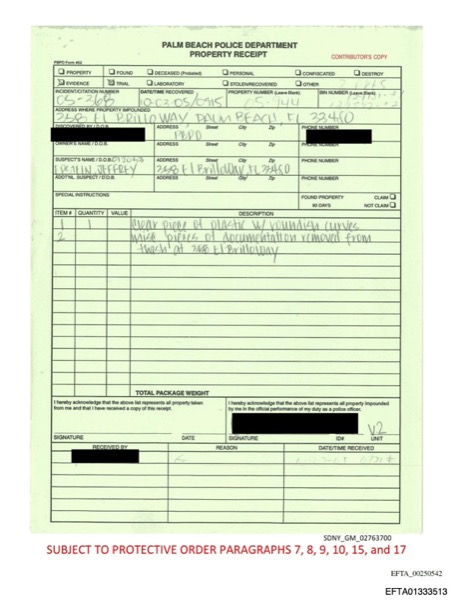
\includegraphics[keepaspectratio,alt={DOJ}]{Images/EFTA01333513_600.jpg}}
\textbar{}
\pandocbounded{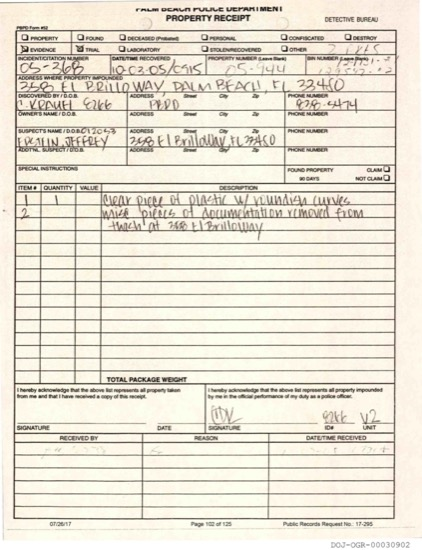
\includegraphics[keepaspectratio,alt={House}]{Images/DOJ-OGR-00030902_550.jpg}}
\textbar{}

Durante lo svolgimento questo progetto, molti utenti hanno pubblicato
programmi e motori di ricerca fatti ad hoc per gli Epstein Files. Uno
dei migliori tra questi, online e molto esauriente,
\href{https://epsteingraph.com/}{è questo}

\paragraph{File Rimossi o Censurati}\label{file-rimossi-o-censurati}

Prima del Epstein Files Transparency Act, ci sono state delle
pubblicazioni giornalistiche di alcuni di questi file, che poi sono
stati pubblicati nei dataset ufficiali.

A complicare la faccenda, il fatto che alcuni documenti sono stati
pubblicati e poi ritirati, perché (o con la scusa che) alcuni di questi
contenevano dati non censurati delle vittime. Esempi di questi dataset
sono: - Il {[}dataset 9{]}
(https://www.justice.gov/epstein/doj-disclosures/data-set-9-files) del
Dipartimento di Giustizia americano consisteva inizialmente in 180 Gb di
files. Per via della presenza di una foto contenente nudi di una vittima
è stato ritirato e poi ripubblicato. Il peso totale dei file, però, è
passato da 180gb a 80gb.
\href{https://www.reddit.com/r/DataHoarder/comments/1qsfv3j/epstein_9_10_11_12_reddit_keeps_nuking_thread_we/}{La
comunità di Reddit} sta cercando di ricreare il dataset - Un insieme di
file presi dai file chiesti e pubblicati dalla Camera statunitense era
stato pubblicato su Hugging Faces sotto il nome di
\href{https://huggingface.co/datasets/tensonaut/EPSTEIN_FILES_20K}{EPSTEIN\_FILES\_20K}.
Gli autori, per le ragioni espresse in
\href{https://www.reddit.com/r/LocalLLaMA/comments/1p4urm7/we_are_considering_removing_the_epstein_files/}{questo
post di Reddit}, hanno deciso di rimuovere il file. Purtroppo, la
maggior parte dei progetti di datascience utilizzavano questo dataset,
che comunque è facilmente scaricabile.

\subparagraph{Cercare tra i File}\label{cercare-tra-i-file}

I dati, così come pubblicati dal DoJ e dalla Camera, sono inutilizzabili
ai fini di analisi di dati. Diversi parsing che usano OCR sono stati
utilizzati per ottenere il testo in formato stringa, in maniera
automatica e senza errori. Questi file, poi, sono stati caricati in rete
e diversi utenti hanno creato browser ad hoc. Un'ottimo motore di
ricercha che utilizza anche dati ottenuti dal parsing è
\href{https://epsteingraph.com/}{questo}

Inoltre,
\href{https://github.com/markramm/EpsteinFiles/blob/main/DOCUMENT_SOURCES.md}{la
pagina github} già citata in precedenza permette di costruire un motore
online. Nel prosimo paragrafo saremo più esaurienti.

\subsubsection{Galassia di Parser per gli Epstein
Files}\label{galassia-di-parser-per-gli-epstein-files}

Vista l'importanza della questione e la natura delle comunity online,
uno zoo di metodi e programmi sono stati sviluppati da utenti in
modalità open source. In seguito un elenco di una (molto piccola) parte
di questi

\paragraph{Parser}\label{parser}

Diversi tipi di parser sono stati implementati. Questi sono ottimi a
dividere i file pubblicati in vari documenti. La maggior parte, oltre a
trasformare l'immagine del testo in una stringa, riconosce i nomi propri
e li salva. Due ottime pagine github sono
\href{https://github.com/markramm/EpsteinFiles}{questa} e
\href{https://github.com/actuallyrizzn/epstein-browser}{questa}

\paragraph{Parser con Riconoscimento
Semantico}\label{parser-con-riconoscimento-semantico}

La faccenda si complica quando si vogliono estrarre relazioni da questi
documenti in formato .txt In questo caso, un'idea possibile, per
procedere in maniera rapida, è quella di chiedere ad un AI di
``leggere'' la mail e di far estrarre a loro le relazioni. Ad esempio
\href{https://github.com/epstein-docs/epstein-docs.github.io}{questa} e
\href{https://github.com/maxandrews/Epstein-doc-explorer}{questa}.
(Quest'ultimo dataset, in particolare, è stato utilizzato per fare
quello che volevo fare io. In gergo tecnico è detto
\href{https://epsteinvisualizer.com/}{``U''})

Sebbene quest'approccio sia tutt'altro che scevro da errori, lo stesso
si può dire per documenti catalogati da umani.

\paragraph{Ranking}\label{ranking}

Un'altra questione importante e strettamente legata alle precedenti è di
ordinare persone e documenti per grado di importanza all'intero dei
file. Alcune pagine hanno implementato un
\href{https://github.com/latent-variable/epstein-ranker}{motore di
ricerca con ranking}.

\href{}{Questo programma filtra le mail e le ordina in base a un
ranking} (del quale non mi occupo in questo progetto ì) \#\#\#\# Altre
risorse interessanti

\href{https://jmail.world}{Le mail di Epstein in formato Gmail (Jmail)}

\subsubsection{Struttura del Report}\label{struttura-del-report}

Il report è organizzato come segue. La Sezione~\ref{sec-dataset}
descrive il dataset, la sua struttura a grafo e le criticità principali.
La \textbf{?@sec-eda} presenta l'analisi esplorativa e la pulizia dei
dati. La \textbf{?@sec-debiasing} discute le strategie di debiasing del
grafo. La \textbf{?@sec-graph-stats} riporta le statistiche di grafo e
le visualizzazioni. Infine, la \textbf{?@sec-ml} presenta gli algoritmi
di machine learning per l'unmasking dei nodi anonimi.

Codice~\ref{lst-documento} Subramonian et al.
(\citeproc{ref-subramonian2024theoretical}{2024}) Andrews
(\citeproc{ref-andrews_epstein_explorer}{2024}) {Jeon et al.}
(\citeproc{ref-jeon2025mitigating}{2025}) Li et al.
(\citeproc{ref-li2023s}{2023}) Shehzad et al.
(\citeproc{ref-shehzad2026graph}{2026}) Healy
(\citeproc{ref-healy_paul_revere_2013}{2013}) Zhang et al.
(\citeproc{ref-zhang2022visual}{2022}) Dı́az et al.
(\citeproc{ref-diaz2024automatic}{2024}) Patel et al.
(\citeproc{ref-patel2012optical}{2012})

\subsection{Dataset}\label{sec-dataset}

Dato il nostro obiettivo

\subsubsection{Descrizione del Dataset}\label{soc-datadescr}

Il dataset che più si avvicina ai miei obiettivi è
\href{https://github.com/maxandrews/Epstein-doc-explorer}{la già citata
pagina github}. I dati consistono in un elenco di triple semantiche
della forma l'\emph{attore} A ha fatto l'\emph{azione} B rivolta al
\emph{target} C presenti negli Epstein Files. Queste relazioni sono
state ottenute utilizzando Claude, e presentano delle incongruenze.

Come da descrizione della pagina github, che ricopio sotto, il dataset è
composto da

\begin{Shaded}
\begin{Highlighting}[]
\CommentTok{{-}{-} Documents table}
\KeywordTok{CREATE} \KeywordTok{TABLE}\NormalTok{ documents (}
  \KeywordTok{id} \DataTypeTok{INTEGER} \KeywordTok{PRIMARY} \KeywordTok{KEY}\NormalTok{ AUTOINCREMENT,}
\NormalTok{  doc\_id TEXT }\KeywordTok{UNIQUE} \KeywordTok{NOT} \KeywordTok{NULL}\NormalTok{,}
\NormalTok{  file\_path TEXT }\KeywordTok{NOT} \KeywordTok{NULL}\NormalTok{,}
\NormalTok{  one\_sentence\_summary TEXT }\KeywordTok{NOT} \KeywordTok{NULL}\NormalTok{,      }\CommentTok{{-}{-} AI{-}generated brief summary}
\NormalTok{  paragraph\_summary TEXT }\KeywordTok{NOT} \KeywordTok{NULL}\NormalTok{,         }\CommentTok{{-}{-} AI{-}generated detailed summary}
\NormalTok{  date\_range\_earliest TEXT,                }\CommentTok{{-}{-} Earliest date mentioned in document}
\NormalTok{  date\_range\_latest TEXT,                  }\CommentTok{{-}{-} Latest date mentioned in document}
  \KeywordTok{category}\NormalTok{ TEXT }\KeywordTok{NOT} \KeywordTok{NULL}\NormalTok{,                  }\CommentTok{{-}{-} Document category}
\NormalTok{  content\_tags TEXT }\KeywordTok{NOT} \KeywordTok{NULL}\NormalTok{,              }\CommentTok{{-}{-} JSON array of content tags}
\NormalTok{  analysis\_timestamp TEXT }\KeywordTok{NOT} \KeywordTok{NULL}\NormalTok{,        }\CommentTok{{-}{-} When analysis was performed}
\NormalTok{  input\_tokens }\DataTypeTok{INTEGER}\NormalTok{,                    }\CommentTok{{-}{-} Claude API usage metrics}
\NormalTok{  output\_tokens }\DataTypeTok{INTEGER}\NormalTok{,}
\NormalTok{  cache\_read\_tokens }\DataTypeTok{INTEGER}\NormalTok{,}
\NormalTok{  cost\_usd }\DataTypeTok{REAL}\NormalTok{,                          }\CommentTok{{-}{-} Estimated API cost}
\NormalTok{  error TEXT,                             }\CommentTok{{-}{-} Error message if analysis failed}
\NormalTok{  created\_at DATETIME }\KeywordTok{DEFAULT} \FunctionTok{CURRENT\_TIMESTAMP}\NormalTok{,}
\NormalTok{  full\_text TEXT                          }\CommentTok{{-}{-} Complete document text for search}
\NormalTok{);}
\KeywordTok{CREATE} \KeywordTok{INDEX}\NormalTok{ idx\_documents\_doc\_id }\KeywordTok{ON}\NormalTok{ documents(doc\_id);}
\KeywordTok{CREATE} \KeywordTok{INDEX}\NormalTok{ idx\_documents\_category }\KeywordTok{ON}\NormalTok{ documents(}\KeywordTok{category}\NormalTok{);}

\CommentTok{{-}{-} RDF triples (relationships)}
\KeywordTok{CREATE} \KeywordTok{TABLE}\NormalTok{ rdf\_triples (}
  \KeywordTok{id} \DataTypeTok{INTEGER} \KeywordTok{PRIMARY} \KeywordTok{KEY}\NormalTok{ AUTOINCREMENT,}
\NormalTok{  doc\_id TEXT }\KeywordTok{NOT} \KeywordTok{NULL}\NormalTok{,}
  \DataTypeTok{timestamp}\NormalTok{ TEXT,                         }\CommentTok{{-}{-} When the event occurred}
\NormalTok{  actor TEXT }\KeywordTok{NOT} \KeywordTok{NULL}\NormalTok{,                    }\CommentTok{{-}{-} Subject of the relationship}
\NormalTok{  action TEXT }\KeywordTok{NOT} \KeywordTok{NULL}\NormalTok{,                   }\CommentTok{{-}{-} Action/verb}
\NormalTok{  target TEXT }\KeywordTok{NOT} \KeywordTok{NULL}\NormalTok{,                   }\CommentTok{{-}{-} Object of the relationship}
\NormalTok{  location TEXT,                          }\CommentTok{{-}{-} Where the event occurred}
\NormalTok{  actor\_likely\_type TEXT,                 }\CommentTok{{-}{-} Type of actor (person, organization, etc.)}
\NormalTok{  triple\_tags TEXT,                       }\CommentTok{{-}{-} JSON array of tags}
\NormalTok{  explicit\_topic TEXT,                    }\CommentTok{{-}{-} Explicit subject matter}
\NormalTok{  implicit\_topic TEXT,                    }\CommentTok{{-}{-} Inferred subject matter}
\NormalTok{  sequence\_order }\DataTypeTok{INTEGER} \KeywordTok{NOT} \KeywordTok{NULL}\NormalTok{,        }\CommentTok{{-}{-} Order within document}
\NormalTok{  top\_cluster\_ids TEXT,                   }\CommentTok{{-}{-} JSON array of top 3 cluster IDs (materialized)}
\NormalTok{  created\_at DATETIME }\KeywordTok{DEFAULT} \FunctionTok{CURRENT\_TIMESTAMP}\NormalTok{,}
  \KeywordTok{FOREIGN} \KeywordTok{KEY}\NormalTok{ (doc\_id) }\KeywordTok{REFERENCES}\NormalTok{ documents(doc\_id) }\KeywordTok{ON} \KeywordTok{DELETE} \KeywordTok{CASCADE}
\NormalTok{);}
\KeywordTok{CREATE} \KeywordTok{INDEX}\NormalTok{ idx\_rdf\_triples\_doc\_id }\KeywordTok{ON}\NormalTok{ rdf\_triples(doc\_id);}
\KeywordTok{CREATE} \KeywordTok{INDEX}\NormalTok{ idx\_rdf\_triples\_actor }\KeywordTok{ON}\NormalTok{ rdf\_triples(actor);}
\KeywordTok{CREATE} \KeywordTok{INDEX}\NormalTok{ idx\_rdf\_triples\_timestamp }\KeywordTok{ON}\NormalTok{ rdf\_triples(}\DataTypeTok{timestamp}\NormalTok{);}
\KeywordTok{CREATE} \KeywordTok{INDEX}\NormalTok{ idx\_top\_cluster\_ids }\KeywordTok{ON}\NormalTok{ rdf\_triples(top\_cluster\_ids);}

\CommentTok{{-}{-} Entity aliases (deduplication)}
\KeywordTok{CREATE} \KeywordTok{TABLE}\NormalTok{ entity\_aliases (}
\NormalTok{  original\_name TEXT }\KeywordTok{PRIMARY} \KeywordTok{KEY}\NormalTok{,}
\NormalTok{  canonical\_name TEXT }\KeywordTok{NOT} \KeywordTok{NULL}\NormalTok{,}
\NormalTok{  reasoning TEXT,                         }\CommentTok{{-}{-} LLM explanation for the merge}
\NormalTok{  created\_at TEXT }\KeywordTok{NOT} \KeywordTok{NULL} \KeywordTok{DEFAULT} \FunctionTok{CURRENT\_TIMESTAMP}\NormalTok{,}
\NormalTok{  created\_by TEXT }\KeywordTok{DEFAULT} \StringTok{\textquotesingle{}llm\_dedupe\textquotesingle{}}    \CommentTok{{-}{-} Source of the alias}
\NormalTok{);}
\end{Highlighting}
\end{Shaded}

\subsubsection{Criticità}\label{criticituxe0}

E' necessario premettere delle osservazioni critiche

\paragraph{Parsing delle Triple
Semantiche}\label{parsing-delle-triple-semantiche}

\paragraph{Diversa Garnularità dei
Document}\label{diversa-garnularituxe0-dei-document}

che valgono per tutti i dataset sugli epstein files. Molti dei files
rilasciati dal DOJ e dalla Camera coincidono. Inoltre, i documenti hanno
una granularità distinta, essendo alcuni libri interi, mentre altri
pagine di documenti.

\paragraph{Deduplicazione}\label{deduplicazione}

In seguito un esempio dello stesso documento presente sotto due diciture
diverse. Per fortuna, non sono presenti duplicati di questo genere nel
nostro dataset.

{\def\LTcaptype{none} % do not increment counter
\begin{longtable}[]{@{}
  >{\centering\arraybackslash}p{(\linewidth - 2\tabcolsep) * \real{0.5000}}
  >{\centering\arraybackslash}p{(\linewidth - 2\tabcolsep) * \real{0.5000}}@{}}
\toprule\noalign{}
\begin{minipage}[b]{\linewidth}\centering
DOJ Released
\end{minipage} & \begin{minipage}[b]{\linewidth}\centering
House Released
\end{minipage} \\
\midrule\noalign{}
\endhead
\bottomrule\noalign{}
\endlastfoot
\pandocbounded{
\includegraphics[keepaspectratio,alt={DOJ}]{Images/EFTA02346130_600.jpg}}
&
\pandocbounded{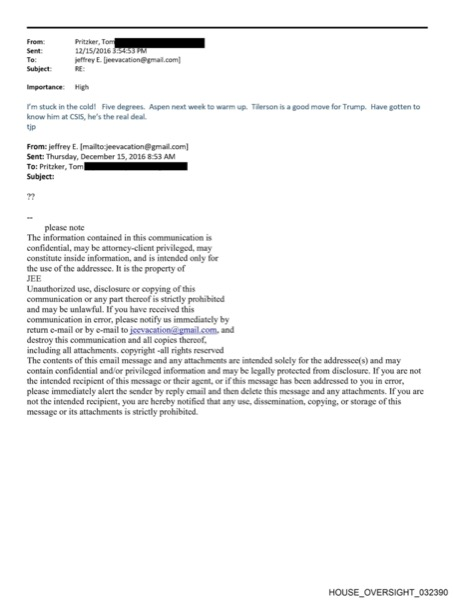
\includegraphics[keepaspectratio,alt={House}]{Images/HOUSE_OVERSIGHT_032390_600.jpg}} \\
\end{longtable}
}

(Una semplice ricerca per data e per nomi porta a
\href{https://www.nytimes.com/2016/12/12/us/politics/rex-tillerson-secretary-of-state-trump.html}{questa
notizia} )

\paragraph{Grado di Bias}\label{grado-di-bias}

\subsection{Exploratory Data Analysis
(EDA)}\label{exploratory-data-analysis-eda}

Iniziamo l'analisi esplorativa importando tutti i pacchetti necessari.

\subsubsection{Upload dei Dati}\label{upload-dei-dati}

Adesso procediamo con l'upload del dataset \textbf{?@sec-datadescr},
salvato in formato .db (database relazionale).

\subsubsection{Pulizia e Filtraggio}\label{pulizia-e-filtraggio}

Procediamo ora a fare una proma pulizia dei dati da inconsistenze e
errori.

\paragraph{Identificazione degli Alias e
un'Inconsistenza}\label{identificazione-degli-alias-e-uninconsistenza}

In primo luogo identifichiamo le identità chiamate con alias diversi. In
secondo luogo andiamo a riempire manualmente un documento ``perduto'', e
cioè un documento che ha dato origine a triple semantiche ma che non è
stato inserito in \texttt{\{python\}documents}. Tale documento può
essere visualizzato in Codice~\ref{lst-documento2}. Infine, rimuoviamo i
documenti che non hanno dato origine a triple semantiche, dato che
questi non verranno utilizzati.

\begin{Shaded}
\begin{Highlighting}[]
\CommentTok{\#{-}{-}{-}{-}{-}{-}{-} PULIZIA PRELIMINARE{-}{-}{-}{-}{-}{-}{-}{-}{-}{-}{-}{-}{-}{-}{-}{-}{-}{-}{-}{-}{-}{-}{-}{-}{-}{-}{-}{-}{-}{-}{-}{-}{-}{-}{-}{-}{-}{-}{-}{-}{-}{-}{-}{-}{-}{-}{-}{-}{-}{-}{-}{-}{-}}
\CommentTok{\#| echo: false}

\CommentTok{\# Deduplichiamo gli alias con cui lo stesso nome è conosciuto}
\CommentTok{\# e.g., \textquotesingle{}Epstein\textquotesingle{} {-}\textgreater{} \textquotesingle{}Jeffrey Epstein\textquotesingle{}.}
\CommentTok{\# }
\CommentTok{\#print(25*\textquotesingle{}{-}\textquotesingle{} +\textquotesingle{} DEDUPLICAZIONE \textquotesingle{} + 25*\textquotesingle{}{-}\textquotesingle{})}
\CommentTok{\#print(\textquotesingle{}Deduplichiamo i nomi canonicizzando i diversi alias\textquotesingle{})}
\NormalTok{alias\_dict }\OperatorTok{=} \BuiltInTok{dict}\NormalTok{(}\BuiltInTok{zip}\NormalTok{(aliases[}\StringTok{"original\_name"}\NormalTok{], aliases[}\StringTok{"canonical\_name"}\NormalTok{])) }\CommentTok{\#Alias dictionary}
\NormalTok{triples[}\StringTok{\textquotesingle{}actor\textquotesingle{}}\NormalTok{] }\OperatorTok{=}\NormalTok{ triples[}\StringTok{\textquotesingle{}actor\textquotesingle{}}\NormalTok{].}\BuiltInTok{map}\NormalTok{(alias\_dict).fillna(triples[}\StringTok{\textquotesingle{}actor\textquotesingle{}}\NormalTok{]) }\CommentTok{\# notice that .map is much faster than .replace}
\NormalTok{triples[}\StringTok{\textquotesingle{}target\textquotesingle{}}\NormalTok{] }\OperatorTok{=}\NormalTok{triples[}\StringTok{\textquotesingle{}target\textquotesingle{}}\NormalTok{].}\BuiltInTok{map}\NormalTok{(alias\_dict).fillna(triples[}\StringTok{\textquotesingle{}target\textquotesingle{}}\NormalTok{])}
\CommentTok{\#print(\textquotesingle{}Deduplicazione completa \textbackslash{}n*\textquotesingle{})}



\CommentTok{\#}
\CommentTok{\# Rimuoviamo i documenti senza triple}
\CommentTok{\#}
\CommentTok{\#print(\textquotesingle{}Filtriamo il dataframe documents prendendo solo \textbackslash{}ni documenti da cui sono state ottenute relazioni semantiche\textquotesingle{})}
\CommentTok{\#print(\textquotesingle{}Molti di questi sono errori o pagine finali di documenti più larghi\textbackslash{}n\textquotesingle{})}
\NormalTok{doc\_ids\_triples }\OperatorTok{=}\NormalTok{ triples[}\StringTok{\textquotesingle{}doc\_id\textquotesingle{}}\NormalTok{].unique()}
\NormalTok{set\_doc\_ids\_triples }\OperatorTok{=} \BuiltInTok{set}\NormalTok{(doc\_ids\_triples)}
\NormalTok{documents }\OperatorTok{=}\NormalTok{ documents[documents[}\StringTok{\textquotesingle{}doc\_id\textquotesingle{}}\NormalTok{].isin(set\_doc\_ids\_triples)]}
\NormalTok{doc\_ids }\OperatorTok{=}\NormalTok{ documents[}\StringTok{\textquotesingle{}doc\_id\textquotesingle{}}\NormalTok{].unique()}
\NormalTok{set\_doc\_ids }\OperatorTok{=} \BuiltInTok{set}\NormalTok{(doc\_ids)}
\CommentTok{\#}
\CommentTok{\# Inconsistenza: Esiste una tripla senza documento!!}
\CommentTok{\#}
\CommentTok{\# Lo andiamo a trovare e lo inseriamo}
\CommentTok{\#print(\textquotesingle{}\textbackslash{}033[1mC\textbackslash{}\textquotesingle{}è un\textbackslash{}inconsistenza nel dataset! \textbackslash{}033[0m\textquotesingle{})}
\CommentTok{\#print(f\textquotesingle{}The number of different documents present in the table doc: \{len(doc\_ids)\}\textquotesingle{})}
\CommentTok{\#print(f\textquotesingle{}The number of different documents present in the table triples: \{len(doc\_ids\_triples)\}\textquotesingle{})}
\CommentTok{\#print(\textquotesingle{}c\textbackslash{}\textquotesingle{}è un documento da cui sono state ottenute triple semantiche che non è inserito nella lista dei documenti\textbackslash{}n\textquotesingle{})}
\CommentTok{\#print(f\textquotesingle{}Il documento è \{set\_doc\_ids\_triples {-} set\_doc\_ids\} \textbackslash{}n\textbackslash{}033[1mNotaì: se la cella viene runnata una seconda volta, l\textbackslash{}\textquotesingle{}inconsistenza sparisce\textbackslash{}033[0m\textbackslash{}n\textquotesingle{})}
\CommentTok{\#print(\textquotesingle{}Il documento può essere trovato quì https://epsteingraph.com/documents/HOUSE\_OVERSIGHT\_013343\textquotesingle{})}
\CommentTok{\#print(\textquotesingle{}Un\textbackslash{}\textquotesingle{}occhiata al documento precedente mostra che le relazioni parsate da esso sono giuste \textquotesingle{})}
\CommentTok{\#print(\textquotesingle{}Decidiamo tenerlo\textquotesingle{})}
\CommentTok{\#print(\textquotesingle{}***** Inseriamo a mano il documento*****\textbackslash{}n\textbackslash{}n\textquotesingle{})}

\NormalTok{category\_documento\_perso }\OperatorTok{=}\NormalTok{ documents[ documents[}\StringTok{\textquotesingle{}doc\_id\textquotesingle{}}\NormalTok{] }\OperatorTok{==}\StringTok{\textquotesingle{}HOUSE\_OVERSIGHT\_013341\textquotesingle{}}\NormalTok{][}\StringTok{\textquotesingle{}category\textquotesingle{}}\NormalTok{].iloc[}\DecValTok{0}\NormalTok{] }\CommentTok{\# Sono pagine di uno stesso documento}
\BuiltInTok{print}\NormalTok{(category\_documento\_perso)}
\NormalTok{documento\_perso }\OperatorTok{=}\NormalTok{ \{}
    \StringTok{\textquotesingle{}doc\_id\textquotesingle{}}\NormalTok{:  }\StringTok{\textquotesingle{}HOUSE\_OVERSIGHT\_013343\textquotesingle{}}\NormalTok{, }
    \StringTok{\textquotesingle{}category\textquotesingle{}}\NormalTok{: }\StringTok{\textquotesingle{}report\textquotesingle{}}\NormalTok{,}\CommentTok{\# A research online shows that froom HOUSE\_OVERSIGHT\_013319 is the sam document, and it is saved here as a report}
    \StringTok{\textquotesingle{}one\_sentence\_summary\textquotesingle{}}\NormalTok{: }\StringTok{\textquotesingle{}Page summarizes allegations that Brunel and the modeling agency MC2, affiliated with Epstein, recruited, housed, and arranged visas for underage girls, reports Brunel visited Epstein in jail approximately 67 times, and cites a June 15, 2010 sworn statement by Maritza Vasquez.\textquotesingle{}}\NormalTok{,}
    \StringTok{\textquotesingle{}full\_text\textquotesingle{}}\NormalTok{: }\StringTok{\textquotesingle{}Edwards that Brunel might have been procuring two eight{-}year{-}old girls for Epstein to sexuallyabuse. According to widely circulated press reports reviewed by Edwards, Brunel is in his sixties and has a reputation throughout the world (and especially in the modeling industry) as a I addict that has for years molested children through modeling agencies while acting as their agent — conduct that has been the subject of critical reports, books, several news articles and a 60 Minutes documentary on Brunel’s sexual exploitation of underage models. See http://bradmillershero.blogspot.com/2010/08/women{-}are{-}objects.html, attached hereto as Exhibit }\CharTok{\textbackslash{}n}\StringTok{ “FE.”}\CharTok{\textbackslash{}n}\StringTok{63. Edwards learned that Brumel is also someone that visited Epstein on approximately 67 occasions while Epstein was in jail. See Epstein}\CharTok{\textbackslash{}\textquotesingle{}}\StringTok{s jail visitor log attached as nd “GG.”}\CharTok{\textbackslash{}n}\StringTok{ 64. Edwards learned that Brunel currently runs the modeling agency MC2, a company for which Epstein provides financial support. See Message Pad}\CharTok{\textbackslash{}\textquotesingle{}}\StringTok{s attached as Exhibit “J” supra Sworn Statement of MC2 employee Maritza Vasquez, June 15, 2010, “Maritza Vasquez Sworn Statement” attached at Exhibit “HH” at 1{-}16.}\CharTok{\textbackslash{}n}\StringTok{ 65. Employees of MC2 told Edwards that Epstein’s numerous condos at 301 East 66 Street in New York were used to house young models. Edwards was told that MC2 modeling agency, affiliated with Epstein and Brunel brought underage girls from all over the world, promising them modeling contracts. Epstein and Brunel would then obtain a visa for these girls, then would charge the underage girls rent, presumably to live as underage prostitutes in the condos. See Maritza Vasquez Sworn Statement, Exhibit “HH” at 7{-}10, 12{-}15, 29{-}30, 39{-}41, 59{-}60 and 62{-}67.}\CharTok{\textbackslash{}n}\StringTok{ 25}\CharTok{\textbackslash{}n}\StringTok{ HOUSE\_OVERSIGHT\_013343\textquotesingle{}}\NormalTok{, }
\NormalTok{\}}
\NormalTok{new\_row\_df }\OperatorTok{=}\NormalTok{ pd.DataFrame([documento\_perso])}
\NormalTok{documents }\OperatorTok{=}\NormalTok{ pd.concat([documents, new\_row\_df], ignore\_index}\OperatorTok{=}\VariableTok{True}\NormalTok{)}
\CommentTok{\#\# The document is not present, but it can be found here. As the }
\CommentTok{\#\# https://epsteingraph.com/documents/HOUSE\_OVERSIGHT\_013343}
\CommentTok{\#print(\textquotesingle{}Documento inserito manualmente\textbackslash{}n Se il programma gira di nuovo, l\textbackslash{}\textquotesingle{}inconsistenza sparisce \textbackslash{}n*\textquotesingle{})}
\CommentTok{\#\#\#\# }
\BuiltInTok{print}\NormalTok{(}\StringTok{"=== Pulizia: Alias e Inconsistenze ==="}\NormalTok{)}
\BuiltInTok{print}\NormalTok{(}\SpecialStringTok{f"Alias canonicalizzati:              }\SpecialCharTok{\{}\BuiltInTok{len}\NormalTok{(alias\_dict)}\SpecialCharTok{\}}\SpecialStringTok{"}\NormalTok{)}
\BuiltInTok{print}\NormalTok{(}\SpecialStringTok{f"Documenti con triple semantiche:    }\SpecialCharTok{\{}\BuiltInTok{len}\NormalTok{(set\_doc\_ids\_triples)}\SpecialCharTok{\}}\SpecialStringTok{"}\NormalTok{)}
\BuiltInTok{print}\NormalTok{(}\SpecialStringTok{f"Documenti nel database:             }\SpecialCharTok{\{}\BuiltInTok{len}\NormalTok{(set\_doc\_ids)}\SpecialCharTok{\}}\SpecialStringTok{"}\NormalTok{)}
\BuiltInTok{print}\NormalTok{(}\SpecialStringTok{f"Inconsistenza trovata:              1 documento mancante (HOUSE\_OVERSIGHT\_013343)"}\NormalTok{)}
\BuiltInTok{print}\NormalTok{(}\SpecialStringTok{f"Azione:                             Inserito manualmente"}\NormalTok{)}
\end{Highlighting}
\end{Shaded}

\begin{verbatim}
court_filing
=== Pulizia: Alias e Inconsistenze ===
Alias canonicalizzati:              28934
Documenti con triple semantiche:    18126
Documenti nel database:             18125
Inconsistenza trovata:              1 documento mancante (HOUSE_OVERSIGHT_013343)
Azione:                             Inserito manualmente
\end{verbatim}

\paragraph{NaN, Deduplicati Forti e Deduplicati
Deboli}\label{nan-deduplicati-forti-e-deduplicati-deboli}

Purtroppo, sono presenti deduplicati deboli, dove per deduplicati deboli
intendiamo documenti identici chiamati con nome diverso, che danno luogo
alle stesse relazioni semantiche. Questi iniziano per TEXT-001 o
TEXT-002- Li andiamo a rimuovere tutti, anche se non tutti sono
duplicati, perché corrispondono a errori

\begin{verbatim}
=== NaN e Duplicati ===
NaN in doc_id:                      0
Duplicati forti (stesso doc_id):    0
Documenti TEXT-* trovati:           2404
Di cui soft duplicates:     2314
Rimuoviamo comunque tutti i documennti che iniziano con TEXT-
\end{verbatim}

\paragraph{Entità Sconosciute e Documentic come
Entità}\label{entituxe0-sconosciute-e-documentic-come-entituxe0}

Le entità sconosciute vengono erroneamente identificate sotto la stessa
entità, mentre, a priori, sono entità distinte. Le rinominiamo in modo
da ottenere entità sconosciute distinte. Inoltre, molte triple sono
erroneamente parsate, essendo l'attore o il target il documento stesso.
Rimuoviamo il documento es inseriamo al suo posto l'altro attore o
l'altro target. Nel caso tutte e due le entità siano documenti,
rimuoviamo la relazione.

Finalmente, inseriamo una colonna con i link ai file in
\href{https://epsteingraph.com/}{questa pagina}.

\begin{verbatim}
Sample Fix: Target 'HOUSE_OVERSIGHT_010734' replaced with 'Kenneth W. Starr' in document 'HOUSE_OVERSIGHT_010734'
Sample Fix: Target 'HOUSE_OVERSIGHT_011163' replaced with 'Unknown_5807' in document 'HOUSE_OVERSIGHT_011163'
Sample Fix: Target 'HOUSE_OVERSIGHT_014130' replaced with 'CONE DENTIAC' in document 'HOUSE_OVERSIGHT_014130'
Sample Fix: Target 'HOUSE_OVERSIGHT_017065' replaced with 'Kurt Bock' in document 'HOUSE_OVERSIGHT_017065'
Sample Fix: Target 'HOUSE_OVERSIGHT_017065' replaced with 'Sergey Brin' in document 'HOUSE_OVERSIGHT_017065'
Sample Fix: Target 'HOUSE_OVERSIGHT_016468' replaced with 'Danny Frost' in document 'HOUSE_OVERSIGHT_016468'
Then we do not have to remove any document
=== Entità Sconosciute e Documenti come Entità ===
Relazioni con attore=documento:     0 → corrette
Relazioni con target=documento:     61 → corrette
Relazioni bidirezionali eliminate:  0
Triple rimanenti:                   92091
Entità 'unknown' rinominate:        17697
\end{verbatim}

\paragraph{Rimozione di Alcuni Dati}\label{rimozione-di-alcuni-dati}

Andiamo a rimuovere i documenti con pochi caratteri. Questi infatti
parsano relazioni sbagliate, visto che molte volte sono le pagine finali
di documenti più ampi. Fissiamo una soglia di 80 caratteri, basata
sull'osservare i documenti formati da un numero inferiore di caratteri.
Rimuoviamo anche le relazioni semantiche associate a tali documenti

\begin{verbatim}
Documenti con meno di 80 caratteri rimossi: 30
Documenti rimanenti: 15692
\end{verbatim}

\paragraph{Pulizia Finale e Risoluzione di
un'Inconsistenza}\label{pulizia-finale-e-risoluzione-di-uninconsistenza}

Procediamo a rimuovere i documenti che non hanno dato luogo ad alcuna
relazione semantica (molti di questi sono stati tolti nel passo
precedente). Scopriamo che esistono relazioni semantiche che non
corrispondono ad alcun documento e andiamo ad aggiumngere il documento
perduto al dataset. Tale documento può essere visualizzato in
Codice~\ref{lst-documento2}

\paragraph{Un'Ulteriore Inconsistenza sulla Categoria di
Documento}\label{unulteriore-inconsistenza-sulla-categoria-di-documento}

(Inoltre, c'è una catgoria che differise solo in un underscore e che
dovrebbero essere considerate le stesse) Notiamo che la categoria di
documento

\begin{verbatim}
Inconsistenza di categoria nei documenti HOUSE_OVERSIGHT_013319–HOUSE_OVERSIGHT_013343:
['court_filing' 'report' 'transcript' 'public record' 'public_record']
(Non corretta — irrilevante per l'analisi)
\end{verbatim}

Altri grafi possono essere trovati
\href{https://epstein-file-explorer.com/network}{qui},
\href{https://epsteingraph.com/}{qui} e \href{}{qui}, gli ultimi due già
studiati precedentemente.

\subsection{Riassunto}\label{riassunto}

\subparagraph{Passaggi logici:}\label{passaggi-logici}

\begin{itemize}
\item
  Analisi esplorativa: Rimuoviamo incongruenze, aggiungiamo dati
  mancanti e rimuoviamo documenti con poco testo
\item
  Visualizzazione: verifichiamo che c'è un cluster di documenti di tipo
  ``book\_excerpt'' con. Questo causa una doppia buca nella
  distribuzione della ``densità di informazione''
\item
  Definizione dei grafi: Definiamo diversi grafi e li esportiamo si
  neo4j
\item
  Analizziamo le metriche standard su ciascuno di essi
\item
  Visualizziamo i cluster di alcuni di essi per vedere che corrispondono
\item ~
  \subparagraph{Progetti Futuri}\label{progetti-futuri}
\item
  Pesare i legami in base al loro valore semantico
\item
  Mantenere un dataset con i documenti, rilasciati ufficialmente e non,
  puliti, deduplicati, indicadone la storia, in formato leggibile e con
  molti metadata.
\item
  insieme ai documenti rilasciati, mantenendo un legame con i file
  originali. Inoltre, mantenere un campo che punta ai duplicati, così da
  poter facilmente rimuovere i duplicati mantenendo la struttura dei
  dataset originali, nella forma in cui sono stati rilasciati (Purtroppo
  la gente non capisce che rendere riproducibili i risultati è l'80\%
  del lavoro. Ci ho messo 4 ore a capire che i file parsati
  \href{https://github.com/epstein-docs/epstein-docs.github.io}{qui}
  provenissero dai
  \href{https://drive.google.com/drive/folders/1TrGxDGQLDLZu1vvvZDBAh-e7wN3y6Hoz}{Documenti
  della Corte Federale statunitense} )
\item
  Migliorare il parsing, soprattutto la parte semantica, per renderlo
  più adatto al nostro scopo
\item
  Applicare tutto ai Panama Papers
\end{itemize}

\paragraph{Consistenza}\label{consistenza}

Dapprima, deduplichiamo i nomi, che, durante il parsing, sono stati
riconosciuti in diverse form, e.g., ``Epstein'', ``Jeff'', ``Jeffrey''..

Dopo procediamo a fare un'analisi di consistenza, nella quale vediamo
che ci sono delle relazioni semantiche trovate in un documento non
presente nel dataset, e cioé il documento `HOUSE\_OVERSIGHT\_013343'.
\href{https://epsteingraph.com/documents/HOUSE_OVERSIGHT_013343}{Una
ricerca in rete} ci fa vedere che le relazioni semantiche sono concordi
con il documento, che provvediamo ad aggiungere al dataset.

Dopodiché filtriamo i documenti che effettivamente hanno dato luogo a
relazioni semantiche. Questi sono errori, documenti pesantemente
censurati, e pagine vuote di documenti più lunghi.

\paragraph{Deduplicazione}\label{deduplicazione-1}

Nel dataset sono presenti dei duplicati ``soft'', che sono stati
scoperti in un secondo momento tramite l'analisi degli outlier della
statistica ``information\_density''. Questi sono documenti che hanno
dato origine ai documenti, e che li contenevano in formato .txt. In
altre parole, sono i file che sono stati processati per dare origine ai
diversi documenti.

Li rimuoviamo facilmente dai documenti, e filtriamo anche le relazioni
semantiche assocuate a questi. Per fortuna, dall'id di questi documenti,
finiti per errore, possiamo possiamo ricavare il loro duplicato e
verificare che effettivamente stiamo rimuovendo duplicati

\paragraph{Pulizia e Visualizzazione}\label{pulizia-e-visualizzazione}

Da un'analisi visiva e individuale dei documenti, rimuoviamo i documenti
il cui testo è inferiore ai 100 caratteri e le loro relazioni semantiche
associate.

Visualizziamo la quantità di documenti presenti per categoria, le triple
semantiche per documento e per argomento esplicito.

Visualizziamo la distribuzione delle lunghezze dei documenti e del
numero di relazioni semantiche associate. Plottiamo, poi, la
distribuzione congiunta di variabili della lunghezza del documento vs
numero di triple semantiche ottenute.

Infine, definiamo la densità di informazione come il numero di triple
semantiche ottenute per 100 caratteri. Verifichiamo che la densità di
informazione dipende dalla grandezza dei documenti considerati. Più
precisamente, fissiamo una sogla treshold (= 2000) e verifichiamo che la
densità di informazione dei diversi documenti con un numero maggiore di
caratteri della soglia ha una distribuzione empirica a doppia buca.
Verifichiamo che questo comportamento e spiegato da un diverso
comportamento della variabile ``information\_density'' rispetto alla
categoria di documenti.

Ipotizziamo, forti dello scatterplot `lunghezza del documenti (in
caratter) vs numero di triple semantiche', che questo è dovuto a una
serie di documenti, in formato di libro o di report, che contengono un
gran numero di caratteri e per cui il numero di relazioni parsate non
cresce di pari passo (in sostanza, danno origine a poche triple
semantiche)

(Più probabilmente dovrei definire la variabile log(densita + 1), ma lo
farò in futuro)

\paragraph{Nota sull'Affidabilità del
Dataset}\label{nota-sullaffidabilituxe0-del-dataset}

Se, da un lato, il lavoro svolto dall'OCR è più affidabile di quello
svolto da un umano, il parsing delle triple semantiche da parte dell'AI
è soggetto a molti errori. Il prossimo chunk di codice mostra che, ad
esempio, il valore alla variabile categoria differisce nonostante i vari
doc\_id si riferiscono a pagine diverse di uno stesso documento.

Per un esempio di validazione di un AI per la validazione di dati
estratti in maniera simile, si osservi l'esempio interessante del grafo
delle triple estratto dai documenti della dittatura di Pinochet
\href{https://arxiv.org/abs/2408.11975}{in questo articolo}

\begin{Shaded}
\begin{Highlighting}[]
\CommentTok{\#\#\# PRIMA VISUALIZZAZIONE}
\NormalTok{n\_documents }\OperatorTok{=} \BuiltInTok{len}\NormalTok{(documents)}
\NormalTok{n\_triples }\OperatorTok{=} \BuiltInTok{len}\NormalTok{(triples)}
\BuiltInTok{print}\NormalTok{(}\StringTok{"=== Statistiche Fondamentali (post{-}pulizia) ==="}\NormalTok{)}
\BuiltInTok{print}\NormalTok{(}\SpecialStringTok{f"Documenti:          }\SpecialCharTok{\{}\NormalTok{n\_documents}\SpecialCharTok{\}}\SpecialStringTok{"}\NormalTok{)}
\BuiltInTok{print}\NormalTok{(}\SpecialStringTok{f"Triple semantiche:  }\SpecialCharTok{\{}\NormalTok{n\_triples}\SpecialCharTok{\}}\SpecialStringTok{"}\NormalTok{)}

\CommentTok{\#print(\textquotesingle{}\textbackslash{}n\textquotesingle{} + 25*\textquotesingle{}{-}\textquotesingle{} +\textquotesingle{} Fundamental Quantities\textquotesingle{} +25*\textquotesingle{}{-}\textquotesingle{}  + \textquotesingle{}\textbackslash{}n\textquotesingle{})}
\CommentTok{\#print(f\textquotesingle{}Il numero di documenti è: \{n\_documents\}\textquotesingle{})}
\CommentTok{\#print(f\textquotesingle{}Il numero di triple è: \{n\_triples\}\textbackslash{}n\textquotesingle{})}

\CommentTok{\# Documenti per gruppo. Categoria}
\CommentTok{\#print(\textquotesingle{}\textbackslash{}n * Il  numero di documenti per categoria \textbackslash{}n\textquotesingle{})}
\BuiltInTok{print}\NormalTok{(documents.groupby(}\StringTok{\textquotesingle{}category\textquotesingle{}}\NormalTok{)[}\StringTok{\textquotesingle{}doc\_id\textquotesingle{}}\NormalTok{].count().sort\_values(ascending }\OperatorTok{=} \VariableTok{False}\NormalTok{).head(}\DecValTok{10}\NormalTok{))}

\CommentTok{\# Numero di documenti per lunghezza}
\CommentTok{\#print(\textquotesingle{}\textbackslash{}n * Il numero di documenti per lunghezza (in unità di 100 caratteri):\textquotesingle{})}
\CommentTok{\#print(\textquotesingle{}Notare che molti documenti sono pagine di documenti più grandi\textbackslash{}n\textquotesingle{})}

\NormalTok{documents[}\StringTok{\textquotesingle{}n\_chars\textquotesingle{}}\NormalTok{] }\OperatorTok{=}\NormalTok{ documents[}\StringTok{\textquotesingle{}full\_text\textquotesingle{}}\NormalTok{].}\BuiltInTok{str}\NormalTok{.}\BuiltInTok{len}\NormalTok{()}\OperatorTok{/}\DecValTok{100} \CommentTok{\# Nuova colonna con la statistica del numero di carateri }

\NormalTok{mean\_value }\OperatorTok{=}\NormalTok{ documents[}\StringTok{\textquotesingle{}n\_chars\textquotesingle{}}\NormalTok{].mean()}
\NormalTok{n\_bins }\OperatorTok{=} \DecValTok{50}

\NormalTok{plt.figure(figsize}\OperatorTok{=}\NormalTok{(}\DecValTok{6}\NormalTok{,}\DecValTok{4}\NormalTok{))}
\NormalTok{sns.histplot(documents[}\StringTok{\textquotesingle{}n\_chars\textquotesingle{}}\NormalTok{], bins }\OperatorTok{=}\NormalTok{ n\_bins, stat }\OperatorTok{=} \StringTok{\textquotesingle{}frequency\textquotesingle{}}\NormalTok{, alpha }\OperatorTok{=} \FloatTok{0.6}\NormalTok{)}
\NormalTok{plt.axvline(mean\_value, color}\OperatorTok{=}\StringTok{\textquotesingle{}red\textquotesingle{}}\NormalTok{, linestyle}\OperatorTok{=}\StringTok{\textquotesingle{}{-}{-}\textquotesingle{}}\NormalTok{, linewidth}\OperatorTok{=}\DecValTok{1}\NormalTok{, label}\OperatorTok{=}\SpecialStringTok{f\textquotesingle{}Mean = }\SpecialCharTok{\{}\NormalTok{mean\_value}\SpecialCharTok{:.2f\}}\SpecialStringTok{\textquotesingle{}}\NormalTok{)}
\CommentTok{\# Labels and title}
\NormalTok{plt.xlabel(}\StringTok{\textquotesingle{}Number of characters\textquotesingle{}}\NormalTok{)}
\NormalTok{plt.ylabel(}\StringTok{\textquotesingle{}Frequency\textquotesingle{}}\NormalTok{)}
\NormalTok{plt.title(}\SpecialStringTok{f\textquotesingle{}Size of the documents in number of characters\textquotesingle{}}\NormalTok{)}
\NormalTok{plt.legend()}
\NormalTok{plt.show()}

\CommentTok{\#\# Tavolazza di colori da usare sempre in  futurp}
\NormalTok{n\_top\_categories }\OperatorTok{=} \DecValTok{4}
\NormalTok{top\_categories }\OperatorTok{=}\NormalTok{ (}
\NormalTok{    documents[}\StringTok{\textquotesingle{}category\textquotesingle{}}\NormalTok{]}
\NormalTok{      .value\_counts()}
\NormalTok{      .head(n\_top\_categories)}
\NormalTok{      .index}
\NormalTok{      .tolist()}
\NormalTok{) }
\NormalTok{colors }\OperatorTok{=}\NormalTok{ sns.color\_palette(}\StringTok{"husl"}\NormalTok{, n\_top\_categories).as\_hex()}
\NormalTok{category\_colors }\OperatorTok{=} \BuiltInTok{dict}\NormalTok{(}\BuiltInTok{zip}\NormalTok{(top\_categories, colors))}

\NormalTok{categorie }\OperatorTok{=}\NormalTok{ [}\StringTok{\textquotesingle{}email\textquotesingle{}}\NormalTok{, }\StringTok{\textquotesingle{}book\_excerpt\textquotesingle{}}\NormalTok{]}
\BuiltInTok{print}\NormalTok{(}\SpecialStringTok{f\textquotesingle{}}\CharTok{\textbackslash{}n}\SpecialStringTok{*Vediamo come cambia la distribuzione delle lunghezze considerando le seguenti diverse categorie }\SpecialCharTok{\{}\NormalTok{categorie}\SpecialCharTok{\}}\SpecialStringTok{\textquotesingle{}}\NormalTok{)}

\NormalTok{mask }\OperatorTok{=}\NormalTok{ documents[}\StringTok{\textquotesingle{}category\textquotesingle{}}\NormalTok{].isin(categorie)}

\NormalTok{doc\_plot }\OperatorTok{=}\NormalTok{ documents[mask]}
\NormalTok{n\_bins }\OperatorTok{=} \DecValTok{60}

\NormalTok{sns.histplot(}
\NormalTok{    data}\OperatorTok{=}\NormalTok{doc\_plot, }
\NormalTok{    x}\OperatorTok{=}\StringTok{\textquotesingle{}n\_chars\textquotesingle{}}\NormalTok{, }
\NormalTok{    hue}\OperatorTok{=}\StringTok{\textquotesingle{}category\textquotesingle{}}\NormalTok{,     }\CommentTok{\# This separates the data by category}
\NormalTok{    bins}\OperatorTok{=}\NormalTok{n\_bins, }
\NormalTok{    palette }\OperatorTok{=}\NormalTok{ category\_colors, }
\NormalTok{    element}\OperatorTok{=}\StringTok{"step"}\NormalTok{,     }\CommentTok{\# \textquotesingle{}step\textquotesingle{} or \textquotesingle{}poly\textquotesingle{} makes overlaps easier to see}
\NormalTok{    stat}\OperatorTok{=}\StringTok{\textquotesingle{}density\textquotesingle{}}\NormalTok{,}
\NormalTok{    common\_norm }\OperatorTok{=} \VariableTok{False}\NormalTok{, }
\NormalTok{    alpha}\OperatorTok{=}\FloatTok{0.4}\NormalTok{,}
\NormalTok{)}

\ControlFlowTok{for}\NormalTok{ cat }\KeywordTok{in}\NormalTok{ categorie:}
    \CommentTok{\# Calculate mean for this specific category}
\NormalTok{    cat\_mean }\OperatorTok{=}\NormalTok{ documents[documents[}\StringTok{\textquotesingle{}category\textquotesingle{}}\NormalTok{] }\OperatorTok{==}\NormalTok{ cat][}\StringTok{\textquotesingle{}n\_chars\textquotesingle{}}\NormalTok{].mean()}
    
    \CommentTok{\# Get the color from our dictionary}
\NormalTok{    line\_color }\OperatorTok{=}\NormalTok{ category\_colors.get(cat)}
    
\NormalTok{    plt.axvline(}
\NormalTok{        x}\OperatorTok{=}\NormalTok{cat\_mean, }
\NormalTok{        color}\OperatorTok{=}\NormalTok{line\_color, }
\NormalTok{        linestyle}\OperatorTok{=}\StringTok{\textquotesingle{}{-}{-}\textquotesingle{}}\NormalTok{, }
\NormalTok{        linewidth}\OperatorTok{=}\FloatTok{1.5}\NormalTok{,}
\NormalTok{        label}\OperatorTok{=}\SpecialStringTok{f\textquotesingle{}Mean }\SpecialCharTok{\{}\NormalTok{cat}\SpecialCharTok{\}}\SpecialStringTok{\textquotesingle{}} \CommentTok{\# Optional: this might make the legend very long}
\NormalTok{    )}

\NormalTok{plt.title(}\SpecialStringTok{f" Grandezza dei documenti in unità di 100 caratteri"}\NormalTok{)}
\NormalTok{plt.show()}
\BuiltInTok{print}\NormalTok{(}\StringTok{\textquotesingle{}Notiamo che la distribuzione dei frammenti di libri sembra essere, a differenza della distribuzione della lunghezza delle mail, distribuita come la somma di due delta, con molti libri molto poco lunghi e un cluster di estratti di libri di 100000 caratteri. Probabilmente questi sono frammenti di un unico libro più grande, ma evitiamo di indagare ulteriormente.\textquotesingle{}}\NormalTok{)}

\CommentTok{\# Numero di triple per documento }
\BuiltInTok{print}\NormalTok{(}\StringTok{\textquotesingle{}}\CharTok{\textbackslash{}n}\StringTok{* Numero di triple per documento: \textquotesingle{}}\NormalTok{)}
\NormalTok{reference\_counts }\OperatorTok{=}\NormalTok{ (}
\NormalTok{    triples.groupby(}\StringTok{\textquotesingle{}doc\_id\textquotesingle{}}\NormalTok{)}
\NormalTok{      .size()}
\NormalTok{      .rename(}\StringTok{\textquotesingle{}n\_triples\textquotesingle{}}\NormalTok{)}
\NormalTok{      .reset\_index()}
\NormalTok{)}
\NormalTok{documents }\OperatorTok{=}\NormalTok{ documents.merge( }\CommentTok{\# Nota, se runnato 2 volte il nome della colonna viene cambiato}
\NormalTok{    reference\_counts,}
\NormalTok{    left\_on}\OperatorTok{=}\StringTok{\textquotesingle{}doc\_id\textquotesingle{}}\NormalTok{,}
\NormalTok{    right\_on}\OperatorTok{=}\StringTok{\textquotesingle{}doc\_id\textquotesingle{}}\NormalTok{,}
\NormalTok{    how}\OperatorTok{=}\StringTok{\textquotesingle{}left\textquotesingle{}}
\NormalTok{).fillna(}\DecValTok{0}\NormalTok{) }\CommentTok{\# Nuova colonna con il numero di triple per ogni documento}
\BuiltInTok{print}\NormalTok{(}\StringTok{\textquotesingle{}}\CharTok{\textbackslash{}n}\StringTok{The number of triples per document}\CharTok{\textbackslash{}n}\StringTok{\textquotesingle{}}\NormalTok{)}
\BuiltInTok{print}\NormalTok{(triples.groupby(}\StringTok{\textquotesingle{}doc\_id\textquotesingle{}}\NormalTok{).size().sort\_values(ascending }\OperatorTok{=} \VariableTok{False}\NormalTok{).head(}\DecValTok{10}\NormalTok{))}

\CommentTok{\# numero di triple per explicit\_topic}
\BuiltInTok{print}\NormalTok{(}\StringTok{\textquotesingle{}}\CharTok{\textbackslash{}n}\StringTok{* Numero di triple per explicit\_topic: \textquotesingle{}}\NormalTok{)}
\BuiltInTok{print}\NormalTok{(triples.groupby(}\StringTok{\textquotesingle{}explicit\_topic\textquotesingle{}}\NormalTok{).size().sort\_values(ascending }\OperatorTok{=} \VariableTok{False}\NormalTok{).head(}\DecValTok{10}\NormalTok{))}

\CommentTok{\#numero di triple per explicit\_topic}
\BuiltInTok{print}\NormalTok{(}\StringTok{\textquotesingle{}}\CharTok{\textbackslash{}n}\StringTok{* Numero di triple per implicit\_topic: \textquotesingle{}}\NormalTok{)}
\BuiltInTok{print}\NormalTok{(triples.groupby(}\StringTok{\textquotesingle{}implicit\_topic\textquotesingle{}}\NormalTok{).size().sort\_values(ascending }\OperatorTok{=} \VariableTok{False}\NormalTok{).head(}\DecValTok{10}\NormalTok{))}



\NormalTok{doc\_plot }\OperatorTok{=}\NormalTok{ documents[documents[}\StringTok{\textquotesingle{}category\textquotesingle{}}\NormalTok{].isin(top\_categories)] }
\NormalTok{sns.scatterplot(}
\NormalTok{    data}\OperatorTok{=}\NormalTok{doc\_plot,}
\NormalTok{    x}\OperatorTok{=}\StringTok{\textquotesingle{}n\_chars\textquotesingle{}}\NormalTok{,}
\NormalTok{    y}\OperatorTok{=}\StringTok{\textquotesingle{}n\_triples\textquotesingle{}}\NormalTok{,}
\NormalTok{    hue}\OperatorTok{=}\StringTok{\textquotesingle{}category\textquotesingle{}}\NormalTok{,             }\CommentTok{\# 👈 Colors by category}
\NormalTok{    palette}\OperatorTok{=}\NormalTok{category\_colors,  }\CommentTok{\# 👈 Plug in your existing palette variable here!}
\NormalTok{    alpha}\OperatorTok{=}\FloatTok{0.7}                   \CommentTok{\# 👈 Makes dots slightly transparent so you can see overlaps}
\NormalTok{)}

\NormalTok{plt.xlabel(}\StringTok{\textquotesingle{}Document Length (Number of Characters)\textquotesingle{}}\NormalTok{)}
\NormalTok{plt.ylabel(}\StringTok{\textquotesingle{}Number of Triples\textquotesingle{}}\NormalTok{)}
\NormalTok{plt.title(}\StringTok{\textquotesingle{}Triples vs. Document Length for Top Categories\textquotesingle{}}\NormalTok{)}

\NormalTok{plt.legend(bbox\_to\_anchor}\OperatorTok{=}\NormalTok{(}\FloatTok{1.05}\NormalTok{, }\DecValTok{1}\NormalTok{), loc}\OperatorTok{=}\StringTok{\textquotesingle{}upper left\textquotesingle{}}\NormalTok{, borderaxespad}\OperatorTok{=}\FloatTok{0.}\NormalTok{)}

\NormalTok{plt.tight\_layout() }
\NormalTok{plt.show()}
\end{Highlighting}
\end{Shaded}

\begin{verbatim}
=== Statistiche Fondamentali (post-pulizia) ===
Documenti:          15692
Triple semantiche:  92058
category
email                 4209
report                2814
book_excerpt          2293
media_article         1695
transcript            1127
financial_document     805
court_filing           667
mixed_document         583
memorandum             400
other                  369
Name: doc_id, dtype: int64
\end{verbatim}

\pandocbounded{\includegraphics[keepaspectratio]{report_files/figure-pdf/cell-11-output-2.png}}

\begin{verbatim}

*Vediamo come cambia la distribuzione delle lunghezze considerando le seguenti diverse categorie ['email', 'book_excerpt']
\end{verbatim}

\pandocbounded{\includegraphics[keepaspectratio]{report_files/figure-pdf/cell-11-output-4.png}}

\begin{verbatim}
Notiamo che la distribuzione dei frammenti di libri sembra essere, a differenza della distribuzione della lunghezza delle mail, distribuita come la somma di due delta, con molti libri molto poco lunghi e un cluster di estratti di libri di 100000 caratteri. Probabilmente questi sono frammenti di un unico libro più grande, ma evitiamo di indagare ulteriormente.

* Numero di triple per documento: 

The number of triples per document

doc_id
HOUSE_OVERSIGHT_017088_part7    107
HOUSE_OVERSIGHT_027594          107
HOUSE_OVERSIGHT_027460          103
HOUSE_OVERSIGHT_022445           85
HOUSE_OVERSIGHT_017088_part4     79
HOUSE_OVERSIGHT_025452           75
HOUSE_OVERSIGHT_020447_part1     70
HOUSE_OVERSIGHT_027165           69
HOUSE_OVERSIGHT_025707           67
HOUSE_OVERSIGHT_023627           67
dtype: int64

* Numero di triple per explicit_topic: 
explicit_topic
confidentiality and privilege notice       106
biographical death notice                   98
ownership interest documentation            89
biographical facts                          77
ownership of confidential communication     67
confidentiality notice                      59
confidentiality disclaimer                  56
ownership claim of communication            42
ownership interest disclosure               41
employment relationship                     41
dtype: int64

* Numero di triple per implicit_topic: 
implicit_topic
relationship cultivation             240
reputation management                187
damage control                       101
legal protection of information       99
legal strategy coordination           98
legal risk mitigation                 94
record of notable deaths              84
political networking                  74
legal protection of communication     56
protecting privileged information     52
dtype: int64
\end{verbatim}

\pandocbounded{\includegraphics[keepaspectratio]{report_files/figure-pdf/cell-11-output-6.png}}

\begin{Shaded}
\begin{Highlighting}[]
\BuiltInTok{print}\NormalTok{(}\DecValTok{25}\OperatorTok{*}\StringTok{\textquotesingle{}{-}\textquotesingle{}} \OperatorTok{+} \StringTok{\textquotesingle{} Bimodalità Densità di Informazione\textquotesingle{}} \OperatorTok{+} \DecValTok{25}\OperatorTok{*}\StringTok{\textquotesingle{}{-}\textquotesingle{}} \OperatorTok{+} \StringTok{\textquotesingle{}}\CharTok{\textbackslash{}n}\StringTok{\textquotesingle{}}\NormalTok{)}
\BuiltInTok{print}\NormalTok{(}\StringTok{\textquotesingle{}\textquotesingle{}\textquotesingle{}Mostriamo che la densità di informazione ha due comportamenti diversi e non è costante }
\StringTok{    rispetto al numero di caratter di un documento}
\StringTok{     \textquotesingle{}\textquotesingle{}\textquotesingle{}}\NormalTok{)}
\BuiltInTok{print}\NormalTok{(}\StringTok{\textquotesingle{}\textquotesingle{}\textquotesingle{}Più precisamente, se consideriamo documenti con un numero di caratteri }
\StringTok{    maggiori di una soglia t, allora la media della densità di informazione decresce.}
\StringTok{     \textquotesingle{}\textquotesingle{}\textquotesingle{}}\NormalTok{)}
\BuiltInTok{print}\NormalTok{(}\StringTok{\textquotesingle{}\textquotesingle{}\textquotesingle{}Se da un lato questo è normale, verifichiamo che questa decrescita dell}\CharTok{\textbackslash{}\textquotesingle{}}\StringTok{informazione }
\StringTok{    non è uniforme lung i gruppi e che da origine ad una distribuzione bimodale della densità }
\StringTok{    di informazione nei documenti}
\StringTok{     \textquotesingle{}\textquotesingle{}\textquotesingle{}}\NormalTok{)}
\BuiltInTok{print}\NormalTok{(}\StringTok{\textquotesingle{}\textquotesingle{}\textquotesingle{}Ipotizziamo, forti dei grafici, che questo fenomeno è dovuto a un cluster di documenti che sono di categoria "book\_excerpt". Non indaghiamo oltre, ma questo diverso comportamento è dovuto al cluster di}
\StringTok{    questo tipo di documento, che si vede nello scatter plot, di poca informazione e gran numero di caratteri. Probabilmente sono pezzi di uno stesso libro più grande, che quindi viene pesato troppo nell}\CharTok{\textbackslash{}\textquotesingle{}}\StringTok{istogramma, ma non indaghiamo oltre.}
\StringTok{     \textquotesingle{}\textquotesingle{}\textquotesingle{}}\NormalTok{)}
\NormalTok{thresholds }\OperatorTok{=}\NormalTok{ [}\DecValTok{15}\NormalTok{,}\DecValTok{25}\NormalTok{,}\DecValTok{35}\NormalTok{] }\CommentTok{\#\# n\_char è in unità di 1000 caratteri. }
\CommentTok{\# Andiamo a filtrare i docuumenti con meno di 1000, 2000, e 3000 caratteri }
\NormalTok{documents[}\StringTok{\textquotesingle{}information\_density\textquotesingle{}}\NormalTok{] }\OperatorTok{=} \DecValTok{100}\OperatorTok{*}\NormalTok{documents[}\StringTok{\textquotesingle{}n\_triples\textquotesingle{}}\NormalTok{]}\OperatorTok{/}\NormalTok{(documents[}\StringTok{\textquotesingle{}n\_chars\textquotesingle{}}\NormalTok{]}\OperatorTok{+}\DecValTok{1}\NormalTok{)}


\CommentTok{\# 1. Setup dimensions}
\NormalTok{coppie\_categorie }\OperatorTok{=} \BuiltInTok{list}\NormalTok{(combinations(top\_categories, }\DecValTok{2}\NormalTok{))}
\NormalTok{n\_rows\_pairs }\OperatorTok{=} \BuiltInTok{len}\NormalTok{(coppie\_categorie)}
\NormalTok{n\_rows\_total }\OperatorTok{=}\NormalTok{ n\_rows\_pairs }\OperatorTok{+} \DecValTok{1} \CommentTok{\# +1 for the Global Row at the top}
\NormalTok{n\_cols }\OperatorTok{=} \BuiltInTok{len}\NormalTok{(thresholds)}

\NormalTok{fig, axes }\OperatorTok{=}\NormalTok{ plt.subplots(n\_rows\_total, n\_cols, figsize}\OperatorTok{=}\NormalTok{(}\DecValTok{7} \OperatorTok{*}\NormalTok{ n\_cols, }\DecValTok{5} \OperatorTok{*}\NormalTok{ n\_rows\_total), constrained\_layout}\OperatorTok{=}\VariableTok{True}\NormalTok{)}

\CommentTok{\# {-}{-}{-} ROW 0: THE GLOBAL DISTRIBUTION (NOT DIVIDED BY CATEGORIES) {-}{-}{-}}
\ControlFlowTok{for}\NormalTok{ col\_idx, threshold }\KeywordTok{in} \BuiltInTok{enumerate}\NormalTok{(thresholds):}
\NormalTok{    ax }\OperatorTok{=}\NormalTok{ axes[}\DecValTok{0}\NormalTok{, col\_idx]}
    
    \CommentTok{\# Filter Total Data}
\NormalTok{    all\_docs\_t }\OperatorTok{=}\NormalTok{ documents[documents[}\StringTok{\textquotesingle{}n\_chars\textquotesingle{}}\NormalTok{] }\OperatorTok{\textgreater{}=}\NormalTok{ threshold]}
\NormalTok{    global\_mean }\OperatorTok{=}\NormalTok{ all\_docs\_t[}\StringTok{\textquotesingle{}information\_density\textquotesingle{}}\NormalTok{].mean()}
    
    \CommentTok{\# Plotting the undivided distribution}
\NormalTok{    sns.histplot(}
\NormalTok{        data}\OperatorTok{=}\NormalTok{all\_docs\_t, x}\OperatorTok{=}\StringTok{\textquotesingle{}information\_density\textquotesingle{}}\NormalTok{, }
\NormalTok{        color}\OperatorTok{=}\StringTok{\textquotesingle{}black\textquotesingle{}}\NormalTok{, element}\OperatorTok{=}\StringTok{"step"}\NormalTok{, stat}\OperatorTok{=}\StringTok{"density"}\NormalTok{, }
\NormalTok{        bins}\OperatorTok{=}\DecValTok{30}\NormalTok{, alpha}\OperatorTok{=}\FloatTok{0.1}\NormalTok{, ax}\OperatorTok{=}\NormalTok{ax, label}\OperatorTok{=}\StringTok{"Undivided Data"}
\NormalTok{    )}
    \CommentTok{\# Adding a solid outline to make the bimodal shape clear}
\NormalTok{    sns.kdeplot(data}\OperatorTok{=}\NormalTok{all\_docs\_t, x}\OperatorTok{=}\StringTok{\textquotesingle{}information\_density\textquotesingle{}}\NormalTok{, color}\OperatorTok{=}\StringTok{\textquotesingle{}black\textquotesingle{}}\NormalTok{, lw}\OperatorTok{=}\DecValTok{2}\NormalTok{, ax}\OperatorTok{=}\NormalTok{ax)}
    
\NormalTok{    ax.axvline(global\_mean, color}\OperatorTok{=}\StringTok{\textquotesingle{}black\textquotesingle{}}\NormalTok{, linestyle}\OperatorTok{=}\StringTok{\textquotesingle{}{-}\textquotesingle{}}\NormalTok{, linewidth}\OperatorTok{=}\DecValTok{2}\NormalTok{)}
\NormalTok{    ax.legend([}\SpecialStringTok{f"Global Mean: }\SpecialCharTok{\{}\NormalTok{global\_mean}\SpecialCharTok{:.2f\}}\SpecialStringTok{"}\NormalTok{], loc}\OperatorTok{=}\StringTok{\textquotesingle{}upper right\textquotesingle{}}\NormalTok{)}
\NormalTok{    ax.set\_title(}\SpecialStringTok{f"GLOBAL DATA (All Categories)}\CharTok{\textbackslash{}n}\SpecialStringTok{Threshold: \textgreater{}}\SpecialCharTok{\{}\NormalTok{threshold}\OperatorTok{*}\DecValTok{100}\SpecialCharTok{\}}\SpecialStringTok{ chars"}\NormalTok{, fontsize}\OperatorTok{=}\DecValTok{12}\NormalTok{, fontweight}\OperatorTok{=}\StringTok{\textquotesingle{}bold\textquotesingle{}}\NormalTok{)}

\CommentTok{\# {-}{-}{-} ROWS 1 to N: CATEGORY PAIRS {-}{-}{-}}
\ControlFlowTok{for}\NormalTok{ row\_idx, pair }\KeywordTok{in} \BuiltInTok{enumerate}\NormalTok{(coppie\_categorie):}
\NormalTok{    current\_row }\OperatorTok{=}\NormalTok{ row\_idx }\OperatorTok{+} \DecValTok{1} \CommentTok{\# Offset by 1 for the global row}
    
    \ControlFlowTok{for}\NormalTok{ col\_idx, threshold }\KeywordTok{in} \BuiltInTok{enumerate}\NormalTok{(thresholds):}
\NormalTok{        ax }\OperatorTok{=}\NormalTok{ axes[current\_row, col\_idx]}

        \CommentTok{\# Filter Data}
\NormalTok{        all\_docs\_t }\OperatorTok{=}\NormalTok{ documents[documents[}\StringTok{\textquotesingle{}n\_chars\textquotesingle{}}\NormalTok{] }\OperatorTok{\textgreater{}=}\NormalTok{ threshold]}
\NormalTok{        cat\_mask }\OperatorTok{=}\NormalTok{ all\_docs\_t[}\StringTok{\textquotesingle{}category\textquotesingle{}}\NormalTok{].isin(pair)}
\NormalTok{        doc\_plot }\OperatorTok{=}\NormalTok{ all\_docs\_t[cat\_mask].copy()}
        
        \CommentTok{\# Overlapping Histograms for the pair}
\NormalTok{        sns.histplot(}
\NormalTok{            data}\OperatorTok{=}\NormalTok{doc\_plot, x}\OperatorTok{=}\StringTok{\textquotesingle{}information\_density\textquotesingle{}}\NormalTok{, hue}\OperatorTok{=}\StringTok{\textquotesingle{}category\textquotesingle{}}\NormalTok{, }
\NormalTok{            hue\_order}\OperatorTok{=}\NormalTok{pair, palette}\OperatorTok{=}\NormalTok{category\_colors,}
\NormalTok{            element}\OperatorTok{=}\StringTok{"step"}\NormalTok{, multiple}\OperatorTok{=}\StringTok{"layer"}\NormalTok{, stat}\OperatorTok{=}\StringTok{"density"}\NormalTok{,     }
\NormalTok{            common\_norm}\OperatorTok{=}\VariableTok{False}\NormalTok{, bins}\OperatorTok{=}\DecValTok{20}\NormalTok{, alpha}\OperatorTok{=}\FloatTok{0.4}\NormalTok{, ax}\OperatorTok{=}\NormalTok{ax, legend}\OperatorTok{=}\VariableTok{False}
\NormalTok{        )}

        \CommentTok{\# Legend with Means and Drops}
\NormalTok{        legend\_elements }\OperatorTok{=}\NormalTok{ []}
        \ControlFlowTok{for}\NormalTok{ cat }\KeywordTok{in}\NormalTok{ pair:}
\NormalTok{            cat\_data }\OperatorTok{=}\NormalTok{ doc\_plot[doc\_plot[}\StringTok{\textquotesingle{}category\textquotesingle{}}\NormalTok{] }\OperatorTok{==}\NormalTok{ cat]}
            \ControlFlowTok{if} \KeywordTok{not}\NormalTok{ cat\_data.empty:}
\NormalTok{                m }\OperatorTok{=}\NormalTok{ cat\_data[}\StringTok{\textquotesingle{}information\_density\textquotesingle{}}\NormalTok{].mean()}
\NormalTok{                c }\OperatorTok{=}\NormalTok{ category\_colors.get(cat)}
\NormalTok{                ax.axvline(m, color}\OperatorTok{=}\NormalTok{c, linestyle}\OperatorTok{=}\StringTok{\textquotesingle{}{-}{-}\textquotesingle{}}\NormalTok{, lw}\OperatorTok{=}\DecValTok{2}\NormalTok{)}
\NormalTok{                legend\_elements.append(Line2D([}\DecValTok{0}\NormalTok{], [}\DecValTok{0}\NormalTok{], color}\OperatorTok{=}\NormalTok{c, lw}\OperatorTok{=}\DecValTok{2}\NormalTok{, linestyle}\OperatorTok{=}\StringTok{\textquotesingle{}{-}{-}\textquotesingle{}}\NormalTok{, }
\NormalTok{                                              label}\OperatorTok{=}\SpecialStringTok{f\textquotesingle{}}\SpecialCharTok{\{}\NormalTok{cat}\SpecialCharTok{\}}\SpecialStringTok{ (μ=}\SpecialCharTok{\{}\NormalTok{m}\SpecialCharTok{:.2f\}}\SpecialStringTok{)\textquotesingle{}}\NormalTok{))}

\NormalTok{        ax.legend(handles}\OperatorTok{=}\NormalTok{legend\_elements, loc}\OperatorTok{=}\StringTok{\textquotesingle{}upper right\textquotesingle{}}\NormalTok{, fontsize}\OperatorTok{=}\DecValTok{8}\NormalTok{)}
\NormalTok{        ax.set\_title(}\SpecialStringTok{f"Pair: }\SpecialCharTok{\{}\NormalTok{pair[}\DecValTok{0}\NormalTok{]}\SpecialCharTok{\}}\SpecialStringTok{ vs }\SpecialCharTok{\{}\NormalTok{pair[}\DecValTok{1}\NormalTok{]}\SpecialCharTok{\}}\SpecialStringTok{"}\NormalTok{, fontsize}\OperatorTok{=}\DecValTok{11}\NormalTok{)}

\NormalTok{plt.suptitle(}\StringTok{\textquotesingle{}Evolution of Bimodal Density: Global Overview vs. Categorical Pairs\textquotesingle{}}\NormalTok{, fontsize}\OperatorTok{=}\DecValTok{22}\NormalTok{, y}\OperatorTok{=}\FloatTok{1.03}\NormalTok{)}
\NormalTok{plt.show()}



\NormalTok{stats\_list }\OperatorTok{=}\NormalTok{ []}

\ControlFlowTok{for}\NormalTok{ t }\KeywordTok{in}\NormalTok{ thresholds:}
    \CommentTok{\# Filter documents based on current threshold}
\NormalTok{    mask\_t }\OperatorTok{=}\NormalTok{ documents[}\StringTok{\textquotesingle{}n\_chars\textquotesingle{}}\NormalTok{] }\OperatorTok{\textgreater{}=}\NormalTok{ t}
\NormalTok{    temp\_df }\OperatorTok{=}\NormalTok{ documents[mask\_t]}
    
    \ControlFlowTok{for}\NormalTok{ cat }\KeywordTok{in}\NormalTok{ top\_categories:}
        \CommentTok{\# Calculate mean for the category at this threshold}
\NormalTok{        cat\_data }\OperatorTok{=}\NormalTok{ temp\_df[temp\_df[}\StringTok{\textquotesingle{}category\textquotesingle{}}\NormalTok{] }\OperatorTok{==}\NormalTok{ cat]}
        \ControlFlowTok{if} \KeywordTok{not}\NormalTok{ cat\_data.empty:}
\NormalTok{            mean\_val }\OperatorTok{=}\NormalTok{ cat\_data[}\StringTok{\textquotesingle{}information\_density\textquotesingle{}}\NormalTok{].mean()}
\NormalTok{            stats\_list.append(\{}
                \StringTok{\textquotesingle{}Threshold (chars)\textquotesingle{}}\NormalTok{: t }\OperatorTok{*} \DecValTok{100}\NormalTok{, }\CommentTok{\# Converting units back to characters}
                \StringTok{\textquotesingle{}Category\textquotesingle{}}\NormalTok{: cat,}
                \StringTok{\textquotesingle{}Mean Density\textquotesingle{}}\NormalTok{: mean\_val,}
                \StringTok{\textquotesingle{}N\textquotesingle{}}\NormalTok{: }\BuiltInTok{len}\NormalTok{(cat\_data)}
\NormalTok{            \})}

\CommentTok{\# Create a summary DataFrame}
\NormalTok{df\_stats }\OperatorTok{=}\NormalTok{ pd.DataFrame(stats\_list)}

 \CommentTok{\# Calculate Global Stats}
\NormalTok{global\_stats }\OperatorTok{=}\NormalTok{ []}
\ControlFlowTok{for}\NormalTok{ t }\KeywordTok{in}\NormalTok{ thresholds:}
\NormalTok{    mask\_t }\OperatorTok{=}\NormalTok{ documents[}\StringTok{\textquotesingle{}n\_chars\textquotesingle{}}\NormalTok{] }\OperatorTok{\textgreater{}=}\NormalTok{ t}
\NormalTok{    global\_mean }\OperatorTok{=}\NormalTok{ documents[mask\_t][}\StringTok{\textquotesingle{}information\_density\textquotesingle{}}\NormalTok{].mean()}
\NormalTok{    global\_stats.append(\{}
        \StringTok{\textquotesingle{}Threshold (chars)\textquotesingle{}}\NormalTok{: t }\OperatorTok{*} \DecValTok{100}\NormalTok{,}
        \StringTok{\textquotesingle{}Category\textquotesingle{}}\NormalTok{: }\StringTok{\textquotesingle{}TOTAL (Global)\textquotesingle{}}\NormalTok{,}
        \StringTok{\textquotesingle{}Mean Density\textquotesingle{}}\NormalTok{: global\_mean}
\NormalTok{    \})}

\NormalTok{df\_global }\OperatorTok{=}\NormalTok{ pd.DataFrame(global\_stats)}

\CommentTok{\# Plotting}
\NormalTok{plt.figure(figsize}\OperatorTok{=}\NormalTok{(}\DecValTok{11}\NormalTok{, }\DecValTok{7}\NormalTok{))}

\CommentTok{\# Plot Categories}
\NormalTok{sns.lineplot(data}\OperatorTok{=}\NormalTok{df\_stats, x}\OperatorTok{=}\StringTok{\textquotesingle{}Threshold (chars)\textquotesingle{}}\NormalTok{, y}\OperatorTok{=}\StringTok{\textquotesingle{}Mean Density\textquotesingle{}}\NormalTok{, }
\NormalTok{             hue}\OperatorTok{=}\StringTok{\textquotesingle{}Category\textquotesingle{}}\NormalTok{, palette}\OperatorTok{=}\NormalTok{category\_colors, marker}\OperatorTok{=}\StringTok{\textquotesingle{}o\textquotesingle{}}\NormalTok{, alpha}\OperatorTok{=}\FloatTok{0.6}\NormalTok{)}

\CommentTok{\# Add the TOTAL line}
\NormalTok{sns.lineplot(data}\OperatorTok{=}\NormalTok{df\_global, x}\OperatorTok{=}\StringTok{\textquotesingle{}Threshold (chars)\textquotesingle{}}\NormalTok{, y}\OperatorTok{=}\StringTok{\textquotesingle{}Mean Density\textquotesingle{}}\NormalTok{, }
\NormalTok{             color}\OperatorTok{=}\StringTok{\textquotesingle{}black\textquotesingle{}}\NormalTok{, linewidth}\OperatorTok{=}\DecValTok{4}\NormalTok{, linestyle}\OperatorTok{=}\StringTok{\textquotesingle{}{-}\textquotesingle{}}\NormalTok{, marker}\OperatorTok{=}\StringTok{\textquotesingle{}s\textquotesingle{}}\NormalTok{, }
\NormalTok{             label}\OperatorTok{=}\StringTok{\textquotesingle{}TOTAL (Global Average)\textquotesingle{}}\NormalTok{, zorder}\OperatorTok{=}\DecValTok{10}\NormalTok{)}

\CommentTok{\# Annotate the Bimodal Insight}
\ControlFlowTok{if} \StringTok{\textquotesingle{}book\_excerpt\textquotesingle{}} \KeywordTok{in}\NormalTok{ top\_categories:}
\NormalTok{    book\_val }\OperatorTok{=}\NormalTok{ df\_stats[df\_stats[}\StringTok{\textquotesingle{}Category\textquotesingle{}}\NormalTok{] }\OperatorTok{==} \StringTok{\textquotesingle{}book\_excerpt\textquotesingle{}}\NormalTok{][}\StringTok{\textquotesingle{}Mean Density\textquotesingle{}}\NormalTok{].iloc[}\OperatorTok{{-}}\DecValTok{1}\NormalTok{]}
\NormalTok{    plt.annotate(}\StringTok{\textquotesingle{}Low{-}Density Peak}\CharTok{\textbackslash{}n}\StringTok{(Driven by Books)\textquotesingle{}}\NormalTok{, }
\NormalTok{                 xy}\OperatorTok{=}\NormalTok{(thresholds[}\OperatorTok{{-}}\DecValTok{1}\NormalTok{]}\OperatorTok{*}\DecValTok{100}\NormalTok{, book\_val), }
\NormalTok{                 xytext}\OperatorTok{=}\NormalTok{(thresholds[}\OperatorTok{{-}}\DecValTok{1}\NormalTok{]}\OperatorTok{*}\DecValTok{100} \OperatorTok{{-}} \DecValTok{500}\NormalTok{, book\_val }\OperatorTok{{-}} \FloatTok{0.5}\NormalTok{),}
\NormalTok{                 arrowprops}\OperatorTok{=}\BuiltInTok{dict}\NormalTok{(facecolor}\OperatorTok{=}\StringTok{\textquotesingle{}black\textquotesingle{}}\NormalTok{, shrink}\OperatorTok{=}\FloatTok{0.05}\NormalTok{), fontsize}\OperatorTok{=}\DecValTok{10}\NormalTok{)}

\NormalTok{plt.title(}\StringTok{\textquotesingle{}Mean Drop Comparison: Individual Categories vs. Total Dataset\textquotesingle{}}\NormalTok{, fontsize}\OperatorTok{=}\DecValTok{15}\NormalTok{)}
\NormalTok{plt.ylabel(}\StringTok{\textquotesingle{}Average Information Density\textquotesingle{}}\NormalTok{)}
\NormalTok{plt.grid(}\VariableTok{True}\NormalTok{, alpha}\OperatorTok{=}\FloatTok{0.3}\NormalTok{)}
\NormalTok{plt.legend(bbox\_to\_anchor}\OperatorTok{=}\NormalTok{(}\FloatTok{1.05}\NormalTok{, }\DecValTok{1}\NormalTok{), loc}\OperatorTok{=}\StringTok{\textquotesingle{}upper left\textquotesingle{}}\NormalTok{)}
\NormalTok{plt.show()}
\end{Highlighting}
\end{Shaded}

\begin{verbatim}
------------------------- Bimodalità Densità di Informazione-------------------------

Mostriamo che la densità di informazione ha due comportamenti diversi e non è costante 
    rispetto al numero di caratter di un documento
     
Più precisamente, se consideriamo documenti con un numero di caratteri 
    maggiori di una soglia t, allora la media della densità di informazione decresce.
     
Se da un lato questo è normale, verifichiamo che questa decrescita dell'informazione 
    non è uniforme lung i gruppi e che da origine ad una distribuzione bimodale della densità 
    di informazione nei documenti
     
Ipotizziamo, forti dei grafici, che questo fenomeno è dovuto a un cluster di documenti che sono di categoria "book_excerpt". Non indaghiamo oltre, ma questo diverso comportamento è dovuto al cluster di
    questo tipo di documento, che si vede nello scatter plot, di poca informazione e gran numero di caratteri. Probabilmente sono pezzi di uno stesso libro più grande, che quindi viene pesato troppo nell'istogramma, ma non indaghiamo oltre.
     
\end{verbatim}

\pandocbounded{\includegraphics[keepaspectratio]{report_files/figure-pdf/cell-12-output-2.png}}

\pandocbounded{\includegraphics[keepaspectratio]{report_files/figure-pdf/cell-12-output-3.png}}

\subsection{Salvataggio del grafo}\label{salvataggio-del-grafo}

Ci dichiariamo soddisfatti della pulizia e dell'indagine preliminare.

\paragraph{Grafo Bipartito}\label{grafo-bipartito}

Adesso, andiamo a definire il grafo bipartito ``Scoppiando'' gli edge e
facendo dell'attributo doc\_id un nodo di tipo diverso. In altre parole,
un nodo ``entità'' è connesso a un documento se e solo se tale nodo
entra come attore in una relazione semantica ottenuta dal documento. Un
edge che collega un documento a una entità è presente se e solo se una
relazione semantica è stata ottenuta da quel documento avente come
target tale entità. (Attenzione: I documenti variano sensibilmente e non
sono ``uniformi'', qualsiasi cosa questo voglia dire. Per esempio, alle
volte sono pagine di un libro più grande, mentre, altre volte, sono
tutto il libro )

Le ragioni per fare questo è che, così facendo, liberiamo gli edge da
una variabile in più. Inoltre, da questo grafo bipartito, possiamo
ottenere il grafo originale e un grafo duale.

\paragraph{Neo4j}\label{neo4j}

Dato che vogliamo che l'analisi sia scalabile, salviamo il nostro grafo
nel database Neo4j, appositamente pensato per grandi reti. Il motivo è
che calcolare metriche la dentro è più rapido e, soprattutto, non
richiede ram. Per mancanza di tempo, non verrà utilizzata (forse per la
dashboard) ma carichiamo il dataset nel cloud neao4j lo stesso, per
sviluppi futuri.

\paragraph{Grafi}\label{grafi}

\begin{enumerate}
\def\labelenumi{\arabic{enumi}.}
\tightlist
\item
  Il grafo delle triple semantiche \texttt{g}. E' il grafo in cui i dati
  sono naturalmente scritti
\item
  Il grafo delle triple semantiche senza Epstein
  \texttt{g\_no\_epstein}. Quà, il nodo Epstein è stato rimosso.
\item
  Grafo Bipartito Originale (\texttt{g\_bi}): Multigrafo diretto che
  mappa 1:1 le relazioni semantiche estratte; ogni arco rappresenta una
  singola azione parsata tra un Documento e un'Entità.
\item
  Grafo Bipartito Semplificato (\texttt{g\_bi\_simple})**: Versione
  ottimizzata e ripulita dai ``super-hub'' (es. Epstein), dove gli archi
  multipli sono collassati in un unico arco pesato, conservando i
  metadati in liste.
\item
  Grafo Duale / Proiezione (\texttt{g\_dual})**: Rete unipartita di soli
  Documenti connessi tra loro se condividono entità; il peso dell'arco è
  il numero di entità comuni. (Anche quà Epstein è stato rimosso).
\end{enumerate}

\begin{verbatim}
Dataset preparato in 0.631439208984375 secondi
Bipartite graph saved to memory in 1.1110868453979492 seconds
184116
92058
\end{verbatim}

\begin{Shaded}
\begin{Highlighting}[]

\CommentTok{\#| eval: false}
\CommentTok{\#| echo: false}
\CommentTok{\#\#\# Salviamo il grafo su neo4j}

\NormalTok{URI }\OperatorTok{=} \StringTok{\textquotesingle{}neo4j+ssc://2462d63d.databases.neo4j.io\textquotesingle{}}
\NormalTok{PASSWORD }\OperatorTok{=} \StringTok{\textquotesingle{}dhCd2UmxGRQBuW{-}HKXWKcO4BDnKs0BMcNKSfi6BeWVk\textquotesingle{}}
\NormalTok{USER }\OperatorTok{=} \StringTok{"neo4j"}

\NormalTok{node\_attributes }\OperatorTok{=}\NormalTok{ [}\StringTok{\textquotesingle{}one\_sentence\_summary\textquotesingle{}}\NormalTok{]}
\NormalTok{edge\_attributes }\OperatorTok{=}\NormalTok{ [}\StringTok{\textquotesingle{}action\textquotesingle{}}\NormalTok{, }\StringTok{\textquotesingle{}original\_edge\_id\textquotesingle{}}\NormalTok{]}
\ControlFlowTok{with}\NormalTok{ GraphDatabase.driver(URI, auth}\OperatorTok{=}\NormalTok{(USER, PASSWORD)) }\ImportTok{as}\NormalTok{ driver:}
\NormalTok{     utl.save\_igraph\_to\_neo4j(driver, g\_bi, node\_attrs }\OperatorTok{=}\NormalTok{ node\_attributes , edge\_attrs }\OperatorTok{=}\NormalTok{ edge\_attributes)}
\end{Highlighting}
\end{Shaded}

\begin{Shaded}
\begin{Highlighting}[]
\CommentTok{\#\#\#\# Let\textquotesingle{}s try to read the graph}

\NormalTok{URI }\OperatorTok{=} \StringTok{\textquotesingle{}neo4j+ssc://2462d63d.databases.neo4j.io\textquotesingle{}}
\NormalTok{PASSWORD }\OperatorTok{=} \StringTok{\textquotesingle{}dhCd2UmxGRQBuW{-}HKXWKcO4BDnKs0BMcNKSfi6BeWVk\textquotesingle{}}
\NormalTok{USER }\OperatorTok{=} \StringTok{"neo4j"}


\ControlFlowTok{with}\NormalTok{ GraphDatabase.driver(URI, auth}\OperatorTok{=}\NormalTok{(USER, PASSWORD)) }\ImportTok{as}\NormalTok{ driver:}
\NormalTok{    g\_downloaded }\OperatorTok{=}\NormalTok{ utl.read\_neo4j\_to\_igraph(driver)}
\end{Highlighting}
\end{Shaded}

\begin{Shaded}
\begin{Highlighting}[]
\CommentTok{\#\# A safety check}
\NormalTok{node\_attributes }\OperatorTok{=}\NormalTok{ [}\StringTok{\textquotesingle{}one\_sentence\_summary\textquotesingle{}}\NormalTok{]}
\NormalTok{edge\_attributes }\OperatorTok{=}\NormalTok{ [}\StringTok{\textquotesingle{}action\textquotesingle{}}\NormalTok{, }\StringTok{\textquotesingle{}original\_edge\_id\textquotesingle{}}\NormalTok{]}
\NormalTok{utl.compare\_graphs(g\_downloaded, g\_bi, node\_attrs }\OperatorTok{=}\NormalTok{ node\_attributes, edge\_attrs }\OperatorTok{=}\NormalTok{ edge\_attributes)}
\BuiltInTok{print}\NormalTok{(g\_downloaded.summary())}
\BuiltInTok{print}\NormalTok{(g\_bi.summary())}
\end{Highlighting}
\end{Shaded}

\begin{Highlighting}
\textcolor{black}{NameError: name 'g\_downloaded' is not defined}
\textcolor{black}{}\textcolor{QuartoInternalColor1}{---------------------------------------------------------------------------}\textcolor{QuartoInternalColor2}{}
\textcolor{QuartoInternalColor2}{}\textcolor{QuartoInternalColor1}{NameError}\textcolor{QuartoInternalColor2}{                                 Traceback (most recent call last)}
\textcolor{QuartoInternalColor2}{Cell }\textcolor{QuartoInternalColor3}{In[9], line 4}\textcolor{QuartoInternalColor2}{}
\textcolor{QuartoInternalColor2}{}\textcolor{QuartoInternalColor4}{      2}\textcolor{QuartoInternalColor2}{ node\_attributes }\textcolor{QuartoInternalColor5}{=}\textcolor{QuartoInternalColor2}{ [}\textcolor{QuartoInternalColor6}{'}\textcolor{QuartoInternalColor2}{}\textcolor{QuartoInternalColor6}{one\_sentence\_summary}\textcolor{QuartoInternalColor2}{}\textcolor{QuartoInternalColor6}{'}\textcolor{QuartoInternalColor2}{]}
\textcolor{QuartoInternalColor2}{}\textcolor{QuartoInternalColor4}{      3}\textcolor{QuartoInternalColor2}{ edge\_attributes }\textcolor{QuartoInternalColor5}{=}\textcolor{QuartoInternalColor2}{ [}\textcolor{QuartoInternalColor6}{'}\textcolor{QuartoInternalColor2}{}\textcolor{QuartoInternalColor6}{action}\textcolor{QuartoInternalColor2}{}\textcolor{QuartoInternalColor6}{'}\textcolor{QuartoInternalColor2}{, }\textcolor{QuartoInternalColor6}{'}\textcolor{QuartoInternalColor2}{}\textcolor{QuartoInternalColor6}{original\_edge\_id}\textcolor{QuartoInternalColor2}{}\textcolor{QuartoInternalColor6}{'}\textcolor{QuartoInternalColor2}{]}
\textcolor{QuartoInternalColor2}{}\textcolor{QuartoInternalColor3}{----> 4}\textcolor{QuartoInternalColor2}{ utl}\textcolor{QuartoInternalColor5}{.}\textcolor{QuartoInternalColor2}{compare\_graphs(}\textcolor{QuartoInternalColor2}{g\_downloaded}\textcolor{QuartoInternalColor2}{, g\_bi, node\_attrs }\textcolor{QuartoInternalColor5}{=}\textcolor{QuartoInternalColor2}{ node\_attributes, edge\_attrs }\textcolor{QuartoInternalColor5}{=}\textcolor{QuartoInternalColor2}{ edge\_attributes)}
\textcolor{QuartoInternalColor2}{}\textcolor{QuartoInternalColor4}{      5}\textcolor{QuartoInternalColor2}{ }\textcolor{QuartoInternalColor7}{print}\textcolor{QuartoInternalColor2}{(g\_downloaded}\textcolor{QuartoInternalColor5}{.}\textcolor{QuartoInternalColor2}{summary())}
\textcolor{QuartoInternalColor2}{}\textcolor{QuartoInternalColor4}{      6}\textcolor{QuartoInternalColor2}{ }\textcolor{QuartoInternalColor7}{print}\textcolor{QuartoInternalColor2}{(g\_bi}\textcolor{QuartoInternalColor5}{.}\textcolor{QuartoInternalColor2}{summary())}
\textcolor{QuartoInternalColor2}{}\textcolor{QuartoInternalColor1}{NameError}\textcolor{QuartoInternalColor2}{: name 'g\_downloaded' is not defined}
\end{Highlighting}

\begin{verbatim}
Clean Graph: 52238 entities, 92058 connections.
Clean Graph: 52238 entities, 59940 connections.
Rimuovendo i doppioni... Il grafo è praticamente un albero (ha pochi cicli)
We have deleted Epstein in 0.09250307083129883 s
Abbiamo collassato gli edge del grafo bipartito via Pandas in 10.21 secondi.
Nodi: 67930, Edges: 120963
\end{verbatim}

\subsection{}\label{section}

\begin{verbatim}
0. Creazione copia di lavoro e rimozione nodi indesiderati...
   'Jeffrey Epstein' rimosso dalla copia. Nodi restanti: 67929

1. Estrazione metadati da g_bi_working...
2. Calcolo della topologia con SciPy...
3. Augmentiamo degli edge proiettati...
4. Costruzione del grafo duale definitivo...

Grafo g_dual finale costruito in 77.72 secondi.
Documenti: 15692 | Connessioni: 4385439
\end{verbatim}

\subsection{Statistiche Di Grafo}\label{statistiche-di-grafo}

Adesso andiamo a definire diversi grafi che vogliamo studiare e diamo
una descrizione generale delle varie metriche che, dato un grafo, si
possono definire.

\paragraph{Grafi}\label{grafi-1}

Consideriamo i seguenti grafi:

\begin{itemize}
\tightlist
\item
  Il grafo bipartito già definito in precedenza
\item
  Il grafo delle relazioni semantiche, dove i nodi sono entità, e cioé
  attori o target, e i legami una relazione semantica del tipo \emph{un
  attore} ha fatto \emph{un'azione} a un \emph{target}.
\item
  Il grafo bipartito in cui i legami multipli sono stati sostituiti da
  uno singolo. In pratica, esiste uno e un solo legame tra un entità e
  un documento se e solo se in tale documento è stata trovata una
  relazione semantica con attore l'entità. Esiste uno e un solo legame
  che unisce un documento e un'entità se e solo se esiste una relazione
  semantica ottenuta dal documento che ha come target l'entità
\item
  Il grafo duale. I nodi sono documenti ed esiste un legame tra due
  documenti se e solo se esiste una relazione semantica nel primo
  documento e una nel secondo documento che condividono un'entità, che
  entra nella prima come target e nella seconda come attore.
\item
  Il grafo delle relazioni semantiche senza Epstein.
\end{itemize}

\paragraph{Metriche}\label{metriche}

\subparagraph{Metriche Globali}\label{metriche-globali}

\begin{itemize}
\tightlist
\item
  Numero di nodi
\item
  Numero di archi
\item
  Densità
\item
  Reciprocità (≈ 0 nei grafi bipartiti perfetti)
\item
  Diametro
\item
  Lunghezza media del percorso
\item
  Numero di componenti
\item
  Spectral Gap \#\#\#\#\# Metirche di Nodo
\item
  Degree (In / Out / Totale)
\item
  PageRank
\item
  Betweenness
\item
  Eigenvector Centrality
\item
  Hubs → Entità influenti (Nel caso bipartito) \#\#\#\#\# Metriche di
  Edge
\end{itemize}

\paragraph{Pipeline}\label{pipeline}

Questo documento descrive il flusso completo di un'analisi di grafi che
verrà applicato ai nostri casi

\begin{itemize}
\item
  Creazione del grafo direzionato tramite \texttt{igraph} a partire da
  DataFrame Pandas o un uploas diretto da Neo4j.
\item
  Estrazione della Componente Gigante\\
  \texttt{extract\_main\_component} Calcolo delle Weakly Connected
  Components (WCC). Motivazione: Evita instabilità nelle metriche
  globali, rende centralità e clustering interpretabili e Riduce il
  costo computazionale.
\item
  Statistiche Globali\\
  \texttt{compute\_global\_statistics}
\item
  Metriche Locali (Nodi e Archi)\\
  \texttt{compute\_and\_store\_metrics}
\item
  Community Detection\\
  \texttt{compute\_communities} Infomap e vettore di Fielder
\end{itemize}

\textbf{Analisi Spettrale} - Calcolo del Laplaciano - Spectral Gap -
Vettore di Fiedler

\begin{itemize}
\tightlist
\item
  Pulizia e Bisezione Spettrale\\
  \texttt{clean\_communities\_and\_bisect} \textbf{Obiettivo:} Rendere
  le comunità analiticamente utilizzabili.
\end{itemize}

Filtro Rumore: Comunità Infomap con meno di \texttt{X} nodi (es. 50) →
assegnate a cluster \texttt{-1}.

Bisezione Spettrale: Conversione del Vettore di Fiedler in attributo
binario.

\begin{Shaded}
\begin{Highlighting}[]
\CommentTok{\# 1. Component Extraction}
\NormalTok{g }\OperatorTok{=}\NormalTok{ extract\_main\_component(g, warning\_threshold}\OperatorTok{=}\FloatTok{0.10}\NormalTok{)}

\CommentTok{\# 2. Add Global Graph Attributes (g["..."])}
\NormalTok{g }\OperatorTok{=}\NormalTok{ compute\_global\_statistics(g)}

\CommentTok{\# 3. Add Node \& Edge Attributes (g.vs["..."], g.es["..."])}
\NormalTok{g }\OperatorTok{=}\NormalTok{ compute\_and\_store\_metrics(g)}

\CommentTok{\# 4. Add Community Attributes}
\NormalTok{g }\OperatorTok{=}\NormalTok{ compute\_communities(g)}

\CommentTok{\# 5. Clean and Bisect}
\NormalTok{g, cleaned\_infomap }\OperatorTok{=}\NormalTok{ clean\_communities\_and\_bisect(g, alpha }\OperatorTok{=} \FloatTok{0.1}\NormalTok{)}
\end{Highlighting}
\end{Shaded}

\subsubsection{📊 Graph Data Dictionary}\label{graph-data-dictionary}

Questo documento descrive in modo preciso gli attributi presenti nel
grafo g e dei file (\texttt{GraphML} e \texttt{Parquet}) al termine
della pipeline di analisi del grafo bipartito direzionato.

\begin{center}\rule{0.5\linewidth}{0.5pt}\end{center}

\paragraph{1 Attributi a Livello di
Grafo}\label{attributi-a-livello-di-grafo}

\emph{(g{[}``\ldots{}''{]})}

Descrivono la struttura macroscopica della \textbf{Giant Weakly
Connected Component (WCC)}.

\begin{itemize}
\item
  \textbf{num\_vertices (int)}\\
  Numero totale di nodi nella componente principale.
\item
  \textbf{num\_edges (int)}\\
  Numero totale di archi nella componente principale.
\item
  \textbf{density (float)}\\
  Rapporto tra archi osservati e archi teoricamente possibili.
\item
  \textbf{reciprocity (float)}\\
  Misura della reciprocità degli archi.\\
  Per un grafo bipartito perfetto direzionato dovrebbe essere
  \textbf{0.0}.
\item
  \textbf{avg\_path\_length (float)}\\
  Lunghezza media dei cammini minimi tra tutte le coppie di nodi
  connessi.
\item
  \textbf{diameter (int)}\\
  Lunghezza del cammino minimo più lungo nella rete.
\item
  \textbf{spectral\_gap (float)}\\
  Secondo autovalore della matrice Laplaciana.\\
  Misura la robustezza e la connettività globale della rete.
\item
  \textbf{louvain\_modularity (float)}\\
  Valore globale di modularità ottenuto tramite algoritmo Louvain.
\item
  \textbf{infomap\_modularity (float)}\\
  Valore globale ottenuto dall'algoritmo Infomap (basato sul flusso
  informativo).
\end{itemize}

\begin{center}\rule{0.5\linewidth}{0.5pt}\end{center}

\paragraph{2 Attributi dei Nodi}\label{attributi-dei-nodi}

\emph{(g.vs{[}``\ldots{}''{]} → nodes.parquet)}

Queste colonne sono presenti nel DataFrame esportato dei nodi.

\subparagraph{🔹 Identità e Layout}\label{identituxe0-e-layout}

\begin{itemize}
\item
  \textbf{name (string)}\\
  Identificativo univoco dell'Entità o Documento.
\item
  \textbf{type (boolean)}\\
  Classe bipartita:

  \begin{itemize}
  \tightlist
  \item
    \texttt{True\ /\ 1} → Documento\\
  \item
    \texttt{False\ /\ 0} → Entità
  \end{itemize}
\item
  \textbf{x, y (float)}\\
  Coordinate 2D pre-calcolate per rendering immediato in Streamlit.
\end{itemize}

\subparagraph{🔹 Importanza /
Centralità}\label{importanza-centralituxe0}

\begin{itemize}
\item
  \textbf{degree\_all (int)}\\
  Numero totale di connessioni.
\item
  \textbf{degree\_in (int)}\\
  Numero di archi entranti.
\item
  \textbf{degree\_out (int)}\\
  Numero di archi uscenti.
\item
  \textbf{pagerank (float)}\\
  Misura di influenza basata sul flusso direzionato.
\item
  \textbf{betweenness (float)}\\
  Frequenza con cui il nodo si trova su cammini minimi (misura di
  ``collo di bottiglia'').
\item
  \textbf{eigenvector (float)}\\
  Influenza basata sulla connessione con nodi a loro volta influenti.
\item
  \textbf{hub\_score (float)}\\
  Score HITS -- alto per Entità che puntano a Documenti rilevanti.
\item
  \textbf{authority\_score (float)}\\
  Score HITS -- alto per Documenti puntati da Entità influenti.
\end{itemize}

\subparagraph{🔹 Struttura e Comunità}\label{struttura-e-comunituxe0}

\begin{itemize}
\item
  \textbf{coreness (int)}\\
  Livello di appartenenza al k-core.
\item
  \textbf{clustering\_coeff (float)}\\
  Coefficiente di clustering locale.
\item
  \textbf{fiedler\_vector (float)}\\
  Coordinata continua derivante dalla decomposizione spettrale.
\item
  \textbf{laplacian\_split (int)}\\
  Versione binarizzata del vettore di Fiedler:

  \begin{itemize}
  \tightlist
  \item
    \texttt{1} se ≥ 0\\
  \item
    \texttt{0} se \textless{} 0
  \end{itemize}
\item
  \textbf{louvain\_cluster (int)}\\
  ID della comunità assegnata da Louvain.
\item
  \textbf{infomap\_cluster (int)}\\
  ID grezzo assegnato da Infomap.
\item
  \textbf{cleaned\_infomap (int)}\\
  Versione filtrata:\\
  comunità troppo piccole vengono assegnate al cluster \texttt{-1}
  (rumore).
\end{itemize}

\begin{center}\rule{0.5\linewidth}{0.5pt}\end{center}

\subparagraph{3. Attributi degli Archi}\label{attributi-degli-archi}

\emph{(g.es{[}``\ldots{}''{]} → edges.parquet)}

Queste colonne sono presenti nel DataFrame esportato degli archi.

\begin{itemize}
\item
  \textbf{source (string)}\\
  Nome del nodo origine (Entità).
\item
  \textbf{target (string)}\\
  Nome del nodo destinazione (Documento).
\item
  \textbf{edge\_betweenness (float)}\\
  Importanza strutturale dell'arco nel connettere parti diverse della
  rete.
\end{itemize}

\begin{center}\rule{0.5\linewidth}{0.5pt}\end{center}

\paragraph{4. Esportazione dei Dati}\label{esportazione-dei-dati}

Al termine della pipeline, il grafo viene esportato in due formati:

\subparagraph{🔹 Esportazione GraphML (Struttura Completa del
Grafo)}\label{esportazione-graphml-struttura-completa-del-grafo}

\begin{Shaded}
\begin{Highlighting}[]
\NormalTok{g\_main.write\_graphml(}\StringTok{"epstein\_main\_component.graphml"}\NormalTok{)}
\end{Highlighting}
\end{Shaded}

\subparagraph{Esportazione in formato
.parquet}\label{esportazione-in-formato-.parquet}

Esportazione di nodi e rispettivi attributi e layout

\begin{Shaded}
\begin{Highlighting}[]
\NormalTok{nodes\_df }\OperatorTok{=}\NormalTok{ pd.DataFrame(g\_main.vs.attributes())}
\NormalTok{nodes\_df.to\_parquet(}\StringTok{"nodes.parquet"}\NormalTok{, index}\OperatorTok{=}\VariableTok{False}\NormalTok{)}
\end{Highlighting}
\end{Shaded}

Esportazione degli archi e dei rispettivi attributi

\begin{Shaded}
\begin{Highlighting}[]
\NormalTok{edges\_df }\OperatorTok{=}\NormalTok{ pd.DataFrame(g\_main.es.attributes())}
\NormalTok{edges\_df.to\_parquet(}\StringTok{"edges.parquet"}\NormalTok{, index}\OperatorTok{=}\VariableTok{False}\NormalTok{)}
\end{Highlighting}
\end{Shaded}

Esportazione degli Attributi di grafo

\begin{Shaded}
\begin{Highlighting}[]
\NormalTok{graph\_stats\_df }\OperatorTok{=}\NormalTok{ pd.DataFrame([\{}
\NormalTok{    k: g\_main[k] }\ControlFlowTok{for}\NormalTok{ k }\KeywordTok{in}\NormalTok{ g\_main.attributes()}
\NormalTok{\}])}

\NormalTok{graph\_stats\_df.to\_parquet(}\StringTok{"graph\_stats.parquet"}\NormalTok{, index}\OperatorTok{=}\VariableTok{False}\NormalTok{)}
\end{Highlighting}
\end{Shaded}

\begin{Shaded}
\begin{Highlighting}[]
\CommentTok{\# Let\textquotesingle{}s study g\_no\_epstein}
\NormalTok{g\_no\_epstein }\OperatorTok{=}\NormalTok{ compute(g\_no\_epstein, export\_name }\OperatorTok{=} \StringTok{"g\_no\_epstein"}\NormalTok{)}
\end{Highlighting}
\end{Shaded}

\begin{Highlighting}
\textcolor{black}{NameError: name 'g\_no\_epstein' is not defined}
\textcolor{black}{}\textcolor{QuartoInternalColor1}{---------------------------------------------------------------------------}\textcolor{QuartoInternalColor2}{}
\textcolor{QuartoInternalColor2}{}\textcolor{QuartoInternalColor1}{NameError}\textcolor{QuartoInternalColor2}{                                 Traceback (most recent call last)}
\textcolor{QuartoInternalColor2}{Cell }\textcolor{QuartoInternalColor3}{In[27], line 2}\textcolor{QuartoInternalColor2}{}
\textcolor{QuartoInternalColor2}{}\textcolor{QuartoInternalColor4}{      1}\textcolor{QuartoInternalColor2}{ }\textcolor{QuartoInternalColor8}{# Let's study g\_no\_epstein}\textcolor{QuartoInternalColor2}{}
\textcolor{QuartoInternalColor2}{}\textcolor{QuartoInternalColor3}{----> 2}\textcolor{QuartoInternalColor2}{ g\_no\_epstein }\textcolor{QuartoInternalColor5}{=}\textcolor{QuartoInternalColor2}{ compute(}\textcolor{QuartoInternalColor2}{g\_no\_epstein}\textcolor{QuartoInternalColor2}{, export\_name }\textcolor{QuartoInternalColor5}{=}\textcolor{QuartoInternalColor2}{ }\textcolor{QuartoInternalColor6}{"}\textcolor{QuartoInternalColor2}{}\textcolor{QuartoInternalColor6}{g\_no\_epstein}\textcolor{QuartoInternalColor2}{}\textcolor{QuartoInternalColor6}{"}\textcolor{QuartoInternalColor2}{)}
\textcolor{QuartoInternalColor2}{}\textcolor{QuartoInternalColor1}{NameError}\textcolor{QuartoInternalColor2}{: name 'g\_no\_epstein' is not defined}
\end{Highlighting}

\begin{Shaded}
\begin{Highlighting}[]
\NormalTok{g\_dual }\OperatorTok{=}\NormalTok{ compute(g\_dual, export\_name }\OperatorTok{=} \StringTok{\textquotesingle{}g\_dual\textquotesingle{}}\NormalTok{) }\CommentTok{\#36 minuti solo per il laplaciano}
\end{Highlighting}
\end{Shaded}

\begin{Shaded}
\begin{Highlighting}[]
\CommentTok{\#\# Stampo su schermo un po\textquotesingle{} di metriche}
\NormalTok{stampa(g\_no\_epstein, }\StringTok{\textquotesingle{}Actor {-}\textgreater{} Target Without Epstein\textquotesingle{}}\NormalTok{)}
\NormalTok{stampa(g, }\StringTok{\textquotesingle{}Actor {-}\textgreater{} Action {-}\textgreater{} Target\textquotesingle{}}\NormalTok{)}
\NormalTok{stampa(g\_dual, }\StringTok{\textquotesingle{}Document {-}\textgreater{} Document Without Epstein\textquotesingle{}}\NormalTok{)}
\NormalTok{stampa(g\_bi\_simple, }\StringTok{\textquotesingle{}Actor {-}\textgreater{} Document {-}\textgreater{} Target Bipartite\textquotesingle{}}\NormalTok{)}
\end{Highlighting}
\end{Shaded}

\paragraph{Conclusione}\label{conclusione}

Adesso vediamo se Chomsky e Andrew stanno nello stesso cluster

Per tenere il Fielders vector, dovrei prima calcolare la componente
connessa massimale

Attenzione: La rappresentazione del grafo è sbagliata, ed è molto più ad
asterisco e sparso di così.

\begin{Shaded}
\begin{Highlighting}[]

\CommentTok{\#| eval: false}
\CommentTok{\#| echo: false}

\CommentTok{\#\# Chomsky sta in cluster diversi dal principe andrea? }
\CommentTok{\#\# La risposta è insoddisfacente perché in questo dataset ci sono poche istanze di Chomsky}
\CommentTok{\#\# Nei nuovi documenti, invece, appare più spesso. }
\NormalTok{good }\OperatorTok{=} \StringTok{"Noam Chomsky"}
\NormalTok{bad }\OperatorTok{=} \StringTok{"Prince Andrew, Duke of York"}  

\ControlFlowTok{for}\NormalTok{ grafo }\KeywordTok{in}\NormalTok{ [g, g\_no\_epstein, g\_simple, g\_bi\_simple]:}
\NormalTok{    cluster\_attr }\OperatorTok{=} \StringTok{"cleaned\_infomap"} \ControlFlowTok{if} \StringTok{"cleaned\_infomap"} \KeywordTok{in}\NormalTok{ grafo.vs.attributes() }\ControlFlowTok{else} \StringTok{"infomap\_cluster"}
    
    \ControlFlowTok{try}\NormalTok{:}
\NormalTok{        v1 }\OperatorTok{=}\NormalTok{ grafo.vs.find(name}\OperatorTok{=}\NormalTok{good).index}
\NormalTok{        v2 }\OperatorTok{=}\NormalTok{ grafo.vs.find(name}\OperatorTok{=}\NormalTok{bad).index}
    \ControlFlowTok{except} \PreprocessorTok{ValueError} \ImportTok{as}\NormalTok{ e:}
        \CommentTok{\# Node not found}
\NormalTok{        missing }\OperatorTok{=}\NormalTok{ good }\ControlFlowTok{if} \BuiltInTok{str}\NormalTok{(e).find(good) }\OperatorTok{!=} \OperatorTok{{-}}\DecValTok{1} \ControlFlowTok{else}\NormalTok{ bad}
        \BuiltInTok{print}\NormalTok{(}\SpecialStringTok{f"⚠️ Node \textquotesingle{}}\SpecialCharTok{\{}\NormalTok{missing}\SpecialCharTok{\}}\SpecialStringTok{\textquotesingle{} not found in this graph, skipping."}\NormalTok{)}
        \ControlFlowTok{continue}
    
\NormalTok{    cluster\_v1 }\OperatorTok{=}\NormalTok{ grafo.vs[v1][cluster\_attr]}
\NormalTok{    cluster\_v2 }\OperatorTok{=}\NormalTok{ grafo.vs[v2][cluster\_attr]}

    \ControlFlowTok{if}\NormalTok{ cluster\_v1 }\OperatorTok{==}\NormalTok{ cluster\_v2:}
        \BuiltInTok{print}\NormalTok{(}\SpecialStringTok{f"✅ \textquotesingle{}}\SpecialCharTok{\{}\NormalTok{good}\SpecialCharTok{\}}\SpecialStringTok{\textquotesingle{} and \textquotesingle{}}\SpecialCharTok{\{}\NormalTok{bad}\SpecialCharTok{\}}\SpecialStringTok{\textquotesingle{} are in the same Infomap cluster (}\SpecialCharTok{\{}\NormalTok{cluster\_v1}\SpecialCharTok{\}}\SpecialStringTok{)."}\NormalTok{)}
    \ControlFlowTok{else}\NormalTok{:}
        \BuiltInTok{print}\NormalTok{(}\SpecialStringTok{f"❌ \textquotesingle{}}\SpecialCharTok{\{}\NormalTok{good}\SpecialCharTok{\}}\SpecialStringTok{\textquotesingle{} (}\SpecialCharTok{\{}\NormalTok{cluster\_v1}\SpecialCharTok{\}}\SpecialStringTok{) and \textquotesingle{}}\SpecialCharTok{\{}\NormalTok{bad}\SpecialCharTok{\}}\SpecialStringTok{\textquotesingle{} (}\SpecialCharTok{\{}\NormalTok{cluster\_v2}\SpecialCharTok{\}}\SpecialStringTok{) are in different Infomap clusters."}\NormalTok{)}
\end{Highlighting}
\end{Shaded}

\begin{Highlighting}
\textcolor{black}{NameError: name 'g' is not defined}
\textcolor{black}{}\textcolor{QuartoInternalColor1}{---------------------------------------------------------------------------}\textcolor{QuartoInternalColor2}{}
\textcolor{QuartoInternalColor2}{}\textcolor{QuartoInternalColor1}{NameError}\textcolor{QuartoInternalColor2}{                                 Traceback (most recent call last)}
\textcolor{QuartoInternalColor2}{Cell }\textcolor{QuartoInternalColor3}{In[28], line 10}\textcolor{QuartoInternalColor2}{}
\textcolor{QuartoInternalColor2}{}\textcolor{QuartoInternalColor4}{      7}\textcolor{QuartoInternalColor2}{ good }\textcolor{QuartoInternalColor5}{=}\textcolor{QuartoInternalColor2}{ }\textcolor{QuartoInternalColor6}{"}\textcolor{QuartoInternalColor2}{}\textcolor{QuartoInternalColor6}{Noam Chomsky}\textcolor{QuartoInternalColor2}{}\textcolor{QuartoInternalColor6}{"}\textcolor{QuartoInternalColor2}{}
\textcolor{QuartoInternalColor2}{}\textcolor{QuartoInternalColor4}{      8}\textcolor{QuartoInternalColor2}{ bad }\textcolor{QuartoInternalColor5}{=}\textcolor{QuartoInternalColor2}{ }\textcolor{QuartoInternalColor6}{"}\textcolor{QuartoInternalColor2}{}\textcolor{QuartoInternalColor6}{Prince Andrew, Duke of York}\textcolor{QuartoInternalColor2}{}\textcolor{QuartoInternalColor6}{"}\textcolor{QuartoInternalColor2}{  }
\textcolor{QuartoInternalColor2}{}\textcolor{QuartoInternalColor3}{---> 10}\textcolor{QuartoInternalColor2}{ }\textcolor{QuartoInternalColor7}{for}\textcolor{QuartoInternalColor2}{ grafo }\textcolor{QuartoInternalColor9}{in}\textcolor{QuartoInternalColor2}{ [}\textcolor{QuartoInternalColor2}{g}\textcolor{QuartoInternalColor2}{, g\_no\_epstein, g\_simple, g\_bi\_simple]:}
\textcolor{QuartoInternalColor2}{}\textcolor{QuartoInternalColor4}{     11}\textcolor{QuartoInternalColor2}{     cluster\_attr }\textcolor{QuartoInternalColor5}{=}\textcolor{QuartoInternalColor2}{ }\textcolor{QuartoInternalColor6}{"}\textcolor{QuartoInternalColor2}{}\textcolor{QuartoInternalColor6}{cleaned\_infomap}\textcolor{QuartoInternalColor2}{}\textcolor{QuartoInternalColor6}{"}\textcolor{QuartoInternalColor2}{ }\textcolor{QuartoInternalColor7}{if}\textcolor{QuartoInternalColor2}{ }\textcolor{QuartoInternalColor6}{"}\textcolor{QuartoInternalColor2}{}\textcolor{QuartoInternalColor6}{cleaned\_infomap}\textcolor{QuartoInternalColor2}{}\textcolor{QuartoInternalColor6}{"}\textcolor{QuartoInternalColor2}{ }\textcolor{QuartoInternalColor9}{in}\textcolor{QuartoInternalColor2}{ grafo}\textcolor{QuartoInternalColor5}{.}\textcolor{QuartoInternalColor2}{vs}\textcolor{QuartoInternalColor5}{.}\textcolor{QuartoInternalColor2}{attributes() }\textcolor{QuartoInternalColor7}{else}\textcolor{QuartoInternalColor2}{ }\textcolor{QuartoInternalColor6}{"}\textcolor{QuartoInternalColor2}{}\textcolor{QuartoInternalColor6}{infomap\_cluster}\textcolor{QuartoInternalColor2}{}\textcolor{QuartoInternalColor6}{"}\textcolor{QuartoInternalColor2}{}
\textcolor{QuartoInternalColor2}{}\textcolor{QuartoInternalColor4}{     13}\textcolor{QuartoInternalColor2}{     }\textcolor{QuartoInternalColor7}{try}\textcolor{QuartoInternalColor2}{:}
\textcolor{QuartoInternalColor2}{}\textcolor{QuartoInternalColor1}{NameError}\textcolor{QuartoInternalColor2}{: name 'g' is not defined}
\end{Highlighting}

\pandocbounded{\includegraphics[keepaspectratio]{report_files/figure-pdf/cell-29-output-1.png}}

\begin{verbatim}
np.int64(92049)
\end{verbatim}

\begin{Highlighting}
\textcolor{black}{NameError: name 'g\_no\_epstein' is not defined}
\textcolor{black}{}\textcolor{QuartoInternalColor1}{---------------------------------------------------------------------------}\textcolor{QuartoInternalColor2}{}
\textcolor{QuartoInternalColor2}{}\textcolor{QuartoInternalColor1}{NameError}\textcolor{QuartoInternalColor2}{                                 Traceback (most recent call last)}
\textcolor{QuartoInternalColor2}{Cell }\textcolor{QuartoInternalColor3}{In[31], line 4}\textcolor{QuartoInternalColor2}{}
\textcolor{QuartoInternalColor2}{}\textcolor{QuartoInternalColor4}{      1}\textcolor{QuartoInternalColor2}{ }\textcolor{QuartoInternalColor8}{#| eval: false}\textcolor{QuartoInternalColor2}{}
\textcolor{QuartoInternalColor2}{}\textcolor{QuartoInternalColor4}{      2}\textcolor{QuartoInternalColor2}{ }\textcolor{QuartoInternalColor8}{#| echo: false}\textcolor{QuartoInternalColor2}{}
\textcolor{QuartoInternalColor2}{}\textcolor{QuartoInternalColor4}{      3}\textcolor{QuartoInternalColor2}{ }\textcolor{QuartoInternalColor8}{# 1. Get your graph data into a DataFrame}\textcolor{QuartoInternalColor2}{}
\textcolor{QuartoInternalColor2}{}\textcolor{QuartoInternalColor3}{----> 4}\textcolor{QuartoInternalColor2}{ df\_nodes }\textcolor{QuartoInternalColor5}{=}\textcolor{QuartoInternalColor2}{ }\textcolor{QuartoInternalColor2}{g\_no\_epstein}\textcolor{QuartoInternalColor2}{}\textcolor{QuartoInternalColor5}{.}\textcolor{QuartoInternalColor2}{get\_vertex\_dataframe()}
\textcolor{QuartoInternalColor2}{}\textcolor{QuartoInternalColor4}{      6}\textcolor{QuartoInternalColor2}{ }\textcolor{QuartoInternalColor8}{# 2. Create the cross-tabulation matrix}\textcolor{QuartoInternalColor2}{}
\textcolor{QuartoInternalColor2}{}\textcolor{QuartoInternalColor4}{      7}\textcolor{QuartoInternalColor2}{ }\textcolor{QuartoInternalColor8}{# Rows will be your Infomap Clusters, Columns will be your Topics}\textcolor{QuartoInternalColor2}{}
\textcolor{QuartoInternalColor2}{}\textcolor{QuartoInternalColor4}{      8}\textcolor{QuartoInternalColor2}{ cross\_table }\textcolor{QuartoInternalColor5}{=}\textcolor{QuartoInternalColor2}{ pd}\textcolor{QuartoInternalColor5}{.}\textcolor{QuartoInternalColor2}{crosstab(index}\textcolor{QuartoInternalColor5}{=}\textcolor{QuartoInternalColor2}{df\_nodes[}\textcolor{QuartoInternalColor6}{'}\textcolor{QuartoInternalColor2}{}\textcolor{QuartoInternalColor6}{infomap\_cluster}\textcolor{QuartoInternalColor2}{}\textcolor{QuartoInternalColor6}{'}\textcolor{QuartoInternalColor2}{], }
\textcolor{QuartoInternalColor2}{}\textcolor{QuartoInternalColor4}{      9}\textcolor{QuartoInternalColor2}{                           columns}\textcolor{QuartoInternalColor5}{=}\textcolor{QuartoInternalColor2}{df\_nodes[}\textcolor{QuartoInternalColor6}{'}\textcolor{QuartoInternalColor2}{}\textcolor{QuartoInternalColor6}{implicit\_topic}\textcolor{QuartoInternalColor2}{}\textcolor{QuartoInternalColor6}{'}\textcolor{QuartoInternalColor2}{])}
\textcolor{QuartoInternalColor2}{}\textcolor{QuartoInternalColor1}{NameError}\textcolor{QuartoInternalColor2}{: name 'g\_no\_epstein' is not defined}
\end{Highlighting}

\begin{Shaded}
\begin{Highlighting}[]

\NormalTok{joined\_df }\OperatorTok{=}\NormalTok{ pd.merge(triples, documents, on}\OperatorTok{=}\StringTok{\textquotesingle{}doc\_id\textquotesingle{}}\NormalTok{, how}\OperatorTok{=}\StringTok{\textquotesingle{}left\textquotesingle{}}\NormalTok{)}
\BuiltInTok{print}\NormalTok{(joined\_df.groupby(}\StringTok{\textquotesingle{}category\textquotesingle{}}\NormalTok{)[}\StringTok{\textquotesingle{}implicit\_topic\textquotesingle{}}\NormalTok{].size())}
\end{Highlighting}
\end{Shaded}

\subsection{Appendici}\label{appendici}

\subsubsection{Appendice A: Architettura del
Progetto}\label{sec-architecture}

Per mantenere una pipeline analitica pulita e riproducibile, questo
progetto separa rigorosamente i dati grezzi, gli script computazionali e
il report finale. La repository è strutturata come segue:

\begin{Shaded}
\begin{Highlighting}[]
\NormalTok{.}
\NormalTok{├── Bibliography/       \# Riferimenti accademici, paper e documentazione citati}
\NormalTok{├── Data/               \# Documenti grezzi e database SQLite elaborati}
\NormalTok{├── Output/             \# Esportazioni della rete (Parquet, GraphML, metriche CSV)}
\NormalTok{├── Presentation/       \# Materiali e slide che riassumono i risultati}
\NormalTok{│   └── Images/         \# Risorse grafiche specifiche per la presentazione}
\NormalTok{├── Report/             \# Jupyter Notebook (report.ipynb) nucleo narrativo dell\textquotesingle{}analisi}
\NormalTok{│   ├── report.ipynb    \# The source file}
\NormalTok{│   ├── report.tex      \# The file knitted by quarto}
\NormalTok{│   └── Images/         \# Risorse immagine statiche utilizzate nel report finale}
\NormalTok{├── src/                \# Moduli Python (es. my\_utils.py) per pulizia dati e algoritmi}
\NormalTok{├── README.md           \# Documentazione principale del progetto}
\NormalTok{├── clean.sh            \# Uno script da applicare al .tex generato da quarto per ottenere il .pdf}
\NormalTok{├── \_quarto.yml         \# Il file con i metadata che usa quarto per knittare a .tex}
\NormalTok{└── requirements.txt    \# Tracciamento delle dipendenze Python}
\end{Highlighting}
\end{Shaded}

Vedere Sezione~\ref{sec-appD} per capire come il report.pdf è stato
generato a partire da report.ipynb

\begin{center}\rule{0.5\linewidth}{0.5pt}\end{center}

\subsubsection{Appendice B: Metodologia e Pipeline dei Dati
(Utils)}\label{sec-utils}

Le complesse operazioni di manipolazione dei dati necessarie per
trasformare i testi legali grezzi di Epstein in una rete matematica sono
state gestite da funzioni di utilità personalizzate situate in
\texttt{src/my\_utils.py}. Di seguito è riportato un riepilogo della
logica analitica principale applicata in background al dataset:

\textbf{\texttt{stampa\_info\_doc()}} * \textbf{Obiettivo:} Verificare
l'accuratezza dell'estrazione dell'IA. * \textbf{Logica:} Prende uno
specifico ID documento e formatta in modo ordinato i suoi metadati, il
riepilogo e le relazioni semantiche estratte
(\texttt{Attore\ -\textgreater{}\ Azione\ -\textgreater{}\ Target}).
Questo permette la verifica manuale delle triple rispetto al testo
grezzo senza ingombrare il notebook principale.

\textbf{\texttt{save\_igraph\_to\_neo4j()} \&
\texttt{read\_neo4j\_to\_igraph()}} * \textbf{Obiettivo:} Archiviazione
e recupero dal database. * \textbf{Logica:} Traduce in modo sicuro
l'oggetto Python \texttt{igraph} in memoria in un Graph Database Neo4j
(preservando gli attributi dinamici di nodi e archi), e viceversa.
Questo garantisce che gli oltre 92.000 archi possano essere archiviati e
interrogati in modo persistente.

\textbf{\texttt{compute\_and\_store\_metrics()}} * \textbf{Obiettivo:}
Identificare attori e documenti strutturalmente significativi. *
\textbf{Logica:} Calcola una suite completa di metriche di teoria dei
grafi (PageRank, Betweenness Centrality, Eigenvector Centrality, HITS
Hubs \& Authorities e k-coreness). Salva questi punteggi direttamente
nei nodi, permettendoci di classificare le entità in base alla loro
influenza strutturale piuttosto che al semplice conteggio delle
occorrenze.

\textbf{\texttt{compute\_communities()} \&
\texttt{clean\_communities\_and\_bisect()}} * \textbf{Obiettivo:}
Rilevare cluster operativi distinti all'interno della rete di Epstein. *
\textbf{Logica:} Esegue molteplici algoritmi di rilevamento delle
comunità, inclusi \textbf{Infomap} (che traccia il flusso della rete
orientata) e \textbf{Louvain}. Incorpora un meccanismo di pulizia
automatizzato che filtra i piccoli cluster di ``rumore'', assegnando
raggruppamenti matematicamente significativi agli attori.

\textbf{\texttt{compute\_layout\_and\_export()}} * \textbf{Obiettivo:}
Preparare la rete per l'analisi visiva ed esterna. * \textbf{Logica:}
Calcola le coordinate 2D normalizzate per l'intero grafo. Sceglie
dinamicamente un layout Bipartito parallelo se il grafo collega
strettamente attori a documenti, o un layout force-directed DrL in caso
contrario. Esporta quindi la rete nei formati veloci \texttt{Parquet} e
\texttt{GraphML} nella cartella \texttt{Output/}.

\textbf{\texttt{visualize\_top1000\_subgraph()}} * \textbf{Obiettivo:}
Visualizzazione web interattiva. * \textbf{Logica:} Filtra la rete
mantenendo solo i 1.000 nodi più centrali (basati sul PageRank) e genera
una rete PyVis HTML interattiva e autonoma, colorata automaticamente in
base alle rispettive comunità Infomap.

\begin{center}\rule{0.5\linewidth}{0.5pt}\end{center}

\subsubsection{Appendice C: Esempio di
Documento}\label{appendice-c-esempio-di-documento}

Vediamo un Epstein File salvato nella variabile documenti.

\begin{codelisting}

\caption{\label{lst-documento}Un esempio di documento}

\centering{

\begin{Shaded}
\begin{Highlighting}[]
\NormalTok{utl.stampa\_info\_doc(documents, triples, }\StringTok{\textquotesingle{}HOUSE\_OVERSIGHT\_032390\textquotesingle{}}\NormalTok{, text }\OperatorTok{=} \VariableTok{True}\NormalTok{)}
\end{Highlighting}
\end{Shaded}

\begin{verbatim}

===================== DOCUMENT ID: HOUSE_OVERSIGHT_032390 ======================

SUMMARY:
An email exchange between Tom Pritzker and Jeffrey Epstein regarding weather, travel plans to Aspen, and commentary on Rex Tillerson's appointment as Secretary of State.

METADATA:
 • Category:   email
 • Date Range: 2016-12-15T08:53:00 to 2016-12-15T15:54:53

------------------------------- PARSED RELATIONS -------------------------------

Found 4 semantic relations (Actor → Action → Target):

.................................. Relation 1 ..................................
 ▶ Jeffrey Epstein sent email to Tom Pritzker
   Location: None
   Tags:     ["email_communication","personal_correspondence","minimal_content_message"]
   Explicit: minimal message exchange with query marker
   Implicit: routine correspondence between contacts

.................................. Relation 2 ..................................
 ▶ Tom Pritzker sent email to Jeffrey Epstein
   Location: None
   Tags:     ["email_communication","personal_correspondence","weather_discussion","travel_planning"]
   Explicit: weather conditions and travel plans
   Implicit: casual personal communication between associates

.................................. Relation 3 ..................................
 ▶ Tom Pritzker commented on appointment of Rex Tillerson
   Location: None
   Tags:     ["political_commentary","government_appointments","executive_appointments","positive_assessment"]
   Explicit: commentary on Secretary of State appointment
   Implicit: political evaluation and professional assessment of government official

.................................. Relation 4 ..................................
 ▶ Tom Pritzker noted professional relationship with Rex Tillerson
   Location: CSIS
   Tags:     ["professional_relationship","institutional_connection","networking","CSIS_association"]
   Explicit: acquaintance through think tank
   Implicit: professional networking and relationship cultivation

================================== FULL TEXT ===================================

From: Pritzker, Tom 
Sent: 12/15/2016 3:54:53_________________________PM 
To: jeffrey E. [jeeyacation@gmail.com] 
Subject: RE: 
Importance: High 
I'm stuck in the cold! Five degrees. Aspen next week to warm up. Tilerson is a good move for Trump. Have gotten to 
know him at CSIS, he's the real deal. 
tjp 
From: jeffrey E. [mailto:jeevacation@gmail.com] 
Sent: Thursday, December 15, 2016 8:53 AM 
To: Pritzker, Tom 
Subject: 
?? 
please note 
The information contained in this communication is 
confidential, may be attorney-client privileged, may 
constitute inside information, and is intended only for 
the use of the addressee. It is the property of 
JEE 
Unauthorized use, disclosure or copying of this 
communication or any part thereof is strictly prohibited 
and may be unlawful. If you have received this 
communication in error, please notify us immediately by 
return e-mail or by e-mail to jeevacation@gmail.com, and 
destroy this communication and all copies thereof, 
including all attachments. copyright -all rights reserved 
The contents of this email message and any attachments are intended solely for the addressee(s) and may 
contain confidential and/or privileged information and may be legally protected from disclosure. If you are not 
the intended recipient of this message or their agent, or if this message has been addressed to you in error, 
please immediately alert the sender by reply email and then delete this message and any attachments. If you are 
not the intended recipient, you are hereby notified that any use, dissemination, copying, or storage of this 
message or its attachments is strictly prohibited. 
HOUSE OVERSIGHT 032390 


================================================================================
\end{verbatim}

}

\end{codelisting}%

\begin{codelisting}

\caption{\label{lst-documento2}Il documento inserito manualmente}

\centering{

\begin{Shaded}
\begin{Highlighting}[]
\NormalTok{utl.stampa\_info\_doc(documents, triples, }\StringTok{\textquotesingle{}HOUSE\_OVERSIGHT\_013343\textquotesingle{}}\NormalTok{, text }\OperatorTok{=} \VariableTok{True}\NormalTok{) }
\end{Highlighting}
\end{Shaded}

\begin{verbatim}

===================== DOCUMENT ID: HOUSE_OVERSIGHT_013343 ======================

SUMMARY:
Page summarizes allegations that Brunel and the modeling agency MC2, affiliated with Epstein, recruited, housed, and arranged visas for underage girls, reports Brunel visited Epstein in jail approximately 67 times, and cites a June 15, 2010 sworn statement by Maritza Vasquez.

METADATA:
 • Category:   report
 • Date Range: nan to nan

------------------------------- PARSED RELATIONS -------------------------------

Found 9 semantic relations (Actor → Action → Target):

.................................. Relation 1 ..................................
 ▶ Jean-Luc Didier Henri-Rene Brunel procured minors for Jeffrey Epstein
   Location: None
   Tags:     ["human_trafficking","sexual_exploitation","underage_prostitution"]
   Explicit: recruitment of minors for sexual abuse
   Implicit: human trafficking for sexual exploitation

.................................. Relation 2 ..................................
 ▶ Jean-Luc Didier Henri-Rene Brunel visited Jeffrey Epstein
   Location: jail
   Tags:     ["jail_visits","association","frequent_contact"]
   Explicit: jail visitation
   Implicit: maintaining association while incarcerated

.................................. Relation 3 ..................................
 ▶ Jean-Luc Didier Henri-Rene Brunel runs MC2 modeling agency
   Location: None
   Tags:     ["agency_management"]
   Explicit: management of modeling agency
   Implicit: control over alleged exploitation network

.................................. Relation 4 ..................................
 ▶ Jeffrey Epstein provides financial support to MC2 modeling agency
   Location: None
   Tags:     ["financial_support","agency_funding"]
   Explicit: financial backing of modeling agency
   Implicit: enabling exploitation operation

.................................. Relation 5 ..................................
 ▶ Jeffrey Epstein used condos to house young models
   Location: New York
   Tags:     ["housing","modeling_exploitation"]
   Explicit: housing of underage models
   Implicit: facilitating sexual exploitation

.................................. Relation 6 ..................................
 ▶ MC2 modeling agency brought unknown minor
   Location: None
   Tags:     ["recruitment","human_trafficking"]
   Explicit: recruitment of underage girls
   Implicit: human trafficking for modeling cover

.................................. Relation 7 ..................................
 ▶ Jeffrey Epstein obtained visa for unknown minor
   Location: None
   Tags:     ["visa_fraud","trafficking"]
   Explicit: visa procurement for minors
   Implicit: facilitating international movement for abuse

.................................. Relation 8 ..................................
 ▶ Jeffrey Epstein charged rent to unknown minor
   Location: None
   Tags:     ["financial_exploitation","rent_charging"]
   Explicit: financial exploitation of minors
   Implicit: profit from sexual exploitation

.................................. Relation 9 ..................................
 ▶ Maritza Vasquez provided sworn statement Jeffrey Epstein
   Location: None
   Tags:     ["witness_testimony","investigative_evidence"]
   Explicit: testimony about exploitation
   Implicit: evidence collection for investigation

================================== FULL TEXT ===================================

Edwards that Brunel might have been procuring two eight-year-old girls for Epstein to sexuallyabuse. According to widely circulated press reports reviewed by Edwards, Brunel is in his sixties and has a reputation throughout the world (and especially in the modeling industry) as a I addict that has for years molested children through modeling agencies while acting as their agent — conduct that has been the subject of critical reports, books, several news articles and a 60 Minutes documentary on Brunel’s sexual exploitation of underage models. See http://bradmillershero.blogspot.com/2010/08/women-are-objects.html, attached hereto as Exhibit 
 “FE.”
63. Edwards learned that Brumel is also someone that visited Epstein on approximately 67 occasions while Epstein was in jail. See Epstein's jail visitor log attached as nd “GG.”
 64. Edwards learned that Brunel currently runs the modeling agency MC2, a company for which Epstein provides financial support. See Message Pad's attached as Exhibit “J” supra Sworn Statement of MC2 employee Maritza Vasquez, June 15, 2010, “Maritza Vasquez Sworn Statement” attached at Exhibit “HH” at 1-16.
 65. Employees of MC2 told Edwards that Epstein’s numerous condos at 301 East 66 Street in New York were used to house young models. Edwards was told that MC2 modeling agency, affiliated with Epstein and Brunel brought underage girls from all over the world, promising them modeling contracts. Epstein and Brunel would then obtain a visa for these girls, then would charge the underage girls rent, presumably to live as underage prostitutes in the condos. See Maritza Vasquez Sworn Statement, Exhibit “HH” at 7-10, 12-15, 29-30, 39-41, 59-60 and 62-67.
 25
 HOUSE_OVERSIGHT_013343

================================================================================
\end{verbatim}

}

\end{codelisting}%

\subsubsection{Appendice D: Qualche Modifica da Fare al .tex in
Output}\label{sec-appD}

Il file .pdf generato da quarto presenta delle problematiche riguardanti
colori, emoji e, più seriamente, immagini. Decidiamo quindi generare
(`knittare') il .tex, effettuare le modifiche su quest'ultimo e
compilare. Le modifiche sono le seguenti

Per quanto riguarda le emoji, inseriamo nell'intestazione del file
\_quarto.yml i seguenti pacchetti latex:
\texttt{\textbackslash{}usepackage\{fontawesome5\}\ \textbackslash{}usepackage\{newunicodechar\}}.
Sempre nello stesso header, inseriamo i rimpiazzi per le emoji.

Per quanto riguada i colori, nel processo in cui quarto produce il file
.tex i colori presenti presenti nel
\texttt{\{python\}print(\textquotesingle{}\textquotesingle{})} non
vengono visualizzati. In particolare, l'output della funzione
\texttt{\{python\}\ utl.stampa\_info\_doc} nel .pdf del report è un po'
confuso. Non abbiamo risolto il problema, e l'environment
\texttt{\{tex\}\ \textbackslash{}begin\{verbatim\}-\/-\/-\textbackslash{}end\{verbatim\}}
del .tex, che contiene il testo degli output dei chuck del notebook,
continua a non tenere conto dei colori.

Per quanto riguarda le immagini, bisogna cambiare la grandezza delle
immagini manualmente nel file .tex prodotto da quarto. Ho creato lo
script \texttt{clean.sh} che mi esegue le seguenti modifiche suggerite
nel file \texttt{Report/report.tex} :

\begin{itemize}
\tightlist
\item
  Sostituire\scriptsize
\end{itemize}

\begin{Shaded}
\begin{Highlighting}[]
\NormalTok{Molti di questi file sono doppioni. Ecco un esempio \textbackslash{}textbar\{\} DOJ}
\NormalTok{Released \textbackslash{}textbar\{\} House Released \textbackslash{}textbar\{\}}
\NormalTok{\textbackslash{}textbar:{-}{-}{-}:\textbackslash{}textbar:{-}{-}{-}:\textbackslash{}textbar\{\} \textbackslash{}textbar\{\}}
\NormalTok{\textbackslash{}pandocbounded\{\textbackslash{}includegraphics[keepaspectratio,alt=\{DOJ\}]\{Images/EFTA01333513\_600.jpg\}\}}
\NormalTok{\textbackslash{}textbar\{\}}
\NormalTok{\textbackslash{}pandocbounded\{\textbackslash{}includegraphics[keepaspectratio,alt=\{House\}]\{Images/DOJ{-}OGR{-}00030902\_550.jpg\}\}}
\NormalTok{\textbackslash{}textbar\{\}}
\end{Highlighting}
\end{Shaded}

\normalsize con \scriptsize

\begin{Shaded}
\begin{Highlighting}[]
\NormalTok{Molti di questi file sono doppioni. Ecco un esempio:}

\NormalTok{\textbackslash{}begin\{table\}[htbp]}
\NormalTok{\textbackslash{}centering}
\NormalTok{\textbackslash{}begin\{tabular\}\{cc\}}
\NormalTok{\textbackslash{}textbf\{DOJ Released\} \& \textbackslash{}textbf\{House Released\} \textbackslash{}\textbackslash{}}
\NormalTok{\textbackslash{}includegraphics[width=0.47\textbackslash{}textwidth]\{Images/EFTA01333513\_600.jpg\} \& \textbackslash{}includegraphics[width=0.43\textbackslash{}textwidth]\{Images/DOJ{-}OGR{-}00030902\_550.jpg\} \textbackslash{}\textbackslash{}}
\NormalTok{\textbackslash{}end\{tabular\}}
\NormalTok{\textbackslash{}caption\{Confronto tra i documenti rilasciati dal DOJ e dalla House.\}}
\NormalTok{\textbackslash{}label\{tab:doppioni\}}
\NormalTok{\textbackslash{}end\{table\}}
\end{Highlighting}
\end{Shaded}

\normalsize

\begin{itemize}
\tightlist
\item
  Sostituire \scriptsize
\end{itemize}

\begin{Shaded}
\begin{Highlighting}[]
\NormalTok{\{\textbackslash{}def\textbackslash{}LTcaptype\{none\} \% do not increment counter}
\NormalTok{\textbackslash{}begin\{longtable\}[]\{@\{\}}
\NormalTok{  \textgreater{}\{\textbackslash{}centering\textbackslash{}arraybackslash\}p\{(\textbackslash{}linewidth {-} 2\textbackslash{}tabcolsep) * \textbackslash{}real\{0.5000\}\}}
\NormalTok{  \textgreater{}\{\textbackslash{}centering\textbackslash{}arraybackslash\}p\{(\textbackslash{}linewidth {-} 2\textbackslash{}tabcolsep) * \textbackslash{}real\{0.5000\}\}@\{\}\}}
\NormalTok{\textbackslash{}toprule\textbackslash{}noalign\{\}}
\NormalTok{\textbackslash{}begin\{minipage\}[b]\{\textbackslash{}linewidth\}\textbackslash{}centering}
\NormalTok{DOJ Released}
\NormalTok{\textbackslash{}end\{minipage\} \& \textbackslash{}begin\{minipage\}[b]\{\textbackslash{}linewidth\}\textbackslash{}centering}
\NormalTok{House Released}
\NormalTok{\textbackslash{}end\{minipage\} \textbackslash{}\textbackslash{}}
\NormalTok{\textbackslash{}midrule\textbackslash{}noalign\{\}}
\NormalTok{\textbackslash{}endhead}
\NormalTok{\textbackslash{}bottomrule\textbackslash{}noalign\{\}}
\NormalTok{\textbackslash{}endlastfoot}
\NormalTok{\textbackslash{}pandocbounded\{\textbackslash{}includegraphics[keepaspectratio,alt=\{DOJ\}]\{Images/EFTA02346130\_600.jpg\}\}}
\NormalTok{\&}
\NormalTok{\textbackslash{}pandocbounded\{\textbackslash{}includegraphics[keepaspectratio,alt=\{House\}]\{Images/HOUSE\_OVERSIGHT\_032390\_600.jpg\}\} \textbackslash{}\textbackslash{}}
\NormalTok{\textbackslash{}end\{longtable\}}
\NormalTok{\}}
\end{Highlighting}
\end{Shaded}

\normalsize con il seguente codice \scriptsize

\begin{Shaded}
\begin{Highlighting}[]
\NormalTok{\textbackslash{}begin\{table\}[htbp]}
\NormalTok{\textbackslash{}centering}
\NormalTok{\textbackslash{}begin\{tabular\}\{cc\}}
\NormalTok{\textbackslash{}textbf\{DOJ Released\} \& \textbackslash{}textbf\{House Released\} \textbackslash{}\textbackslash{}}
\NormalTok{\textbackslash{}includegraphics[width=0.45\textbackslash{}textwidth]\{Images/EFTA02346130\_600.jpg\} \& \textbackslash{}includegraphics[width=0.45\textbackslash{}textwidth]\{Images/HOUSE\_OVERSIGHT\_032390\_600.jpg\} \textbackslash{}\textbackslash{}}
\NormalTok{\textbackslash{}end\{tabular\}}
\NormalTok{\textbackslash{}caption\{Confronto tra i documenti rilasciati dal DOJ e dalla House.\}}
\NormalTok{\textbackslash{}label\{tab:doppioni\}}
\NormalTok{\textbackslash{}end\{table\}}
\end{Highlighting}
\end{Shaded}

\normalsize

\protect\phantomsection\label{refs}
\begin{CSLReferences}{1}{0}
\bibitem[\citeproctext]{ref-andrews_epstein_explorer}
Andrews, M. (2024). Epstein Document Explorer. In \emph{GitHub
repository} {[}Software{]}. GitHub.
\url{https://github.com/maxandrews/Epstein-doc-explorer}

\bibitem[\citeproctext]{ref-diaz2024automatic}
Dı́az, C., Dunstan, J., Etcheverry, L., Fonck, A., Grez, A., Mery, D.,
Reutter, J., \& Rojas, H. (2024). Automatic knowledge-graph creation
from historical documents: The Chilean dictatorship as a case study.
\emph{arXiv preprint arXiv:2408.11975}.

\bibitem[\citeproctext]{ref-healy_paul_revere_2013}
Healy, K. (2013). \emph{Using Metadata to Find {Paul Revere}}.
\url{https://kieranhealy.org/blog/archives/2013/06/09/using-metadata-to-find-paul-revere/}

\bibitem[\citeproctext]{ref-jeon2025mitigating}
{Jeon, H.-J., Lee, O.-J., et al.} (2025). Mitigating degree bias in
graph representation learning with learnable structural augmentation and
structural self-attention. \emph{IEEE Transactions on Network Science
and Engineering}.

\bibitem[\citeproctext]{ref-li2023s}
Li, J., Wu, R., Sun, W., Chen, L., Tian, S., Zhu, L., Meng, C., Zheng,
Z., \& Wang, W. (2023). What's behind the mask: Understanding masked
graph modeling for graph autoencoders. \emph{Proceedings of the 29th ACM
SIGKDD conference on knowledge discovery and data mining}, 1268--1279.

\bibitem[\citeproctext]{ref-patel2012optical}
Patel, C., Patel, A., \& Patel, D. (2012). Optical character recognition
by open source OCR tool tesseract: A case study. \emph{International
journal of computer applications}, \emph{55}(10), 50--56.

\bibitem[\citeproctext]{ref-shehzad2026graph}
Shehzad, A., Xia, F., Abid, S., Peng, C., Yu, S., Zhang, D., \&
Verspoor, K. (2026). Graph transformers: A survey. \emph{IEEE
Transactions on Neural Networks and Learning Systems}.

\bibitem[\citeproctext]{ref-subramonian2024theoretical}
Subramonian, A., Kang, J., \& Sun, Y. (2024). Theoretical and empirical
insights into the origins of degree bias in graph neural networks.
\emph{Advances in Neural Information Processing Systems}, \emph{37},
8193--8239.

\bibitem[\citeproctext]{ref-zhang2022visual}
Zhang, W., Tan, S., Chen, S., Meng, L., Zhang, T., Zhu, R., \& Chen, W.
(2022). Visual reasoning for uncertainty in spatio-temporal events of
historical figures. \emph{IEEE Transactions on Visualization and
Computer Graphics}, \emph{29}(6), 3009--3023.

\end{CSLReferences}




\end{document}
